\documentclass[11pt,oneside]{book}

\usepackage[french]{babel}
\usepackage[utf8]{inputenc}  
\usepackage[T1]{fontenc}
\usepackage{listings}
\usepackage{comment}
\usepackage[left=2.5cm,right=2.5cm,top=3cm,bottom=2.65cm]{geometry}
\usepackage{graphicx}
\usepackage{tabularx}
\usepackage{amsmath,amssymb,amsfonts}
\usepackage{bbm, bm}
\usepackage{stmaryrd}
\usepackage{mathtools}
\usepackage{hyperref}
\usepackage{tikz}
\usepackage{tabularx}
\usepackage{makecell}
\usepackage{color}
\usepackage{fancybox}
\usepackage[thmmarks,amsmath]{ntheorem}
\usepackage{minitoc}
\usepackage{titletoc}
\usepackage{tikz}
\usepackage{algpseudocode}
\usepackage[]{algorithm2e}
\usepackage{wrapfig}
\usepackage{kpfonts}

\graphicspath{{images/}}

\DeclareMathOperator*{\argmax}{arg\,max}
\DeclareMathOperator*{\argmin}{arg\,min}

\usetikzlibrary{arrows.meta}
\usetikzlibrary{arrows}
\usetikzlibrary{decorations.pathreplacing}
\mathtoolsset{showonlyrefs=true}

\addto\extrasfrench{%
	\def\subsectionautorefname{\S}%
	\def\sectionautorefname{\S}%
}

\definecolor{darkWhite}{rgb}{0.94,0.94,0.94}
\definecolor{blue}{rgb}{0.12,0.16,0.53}
\definecolor{green}{rgb}{0.25,0.28,0.06}
\definecolor{purple}{rgb}{0.5, 0.1, 0.5}
\definecolor{yellow}{rgb}{0.8, 0.7, 0.1}
\definecolor{greenTikz}{rgb}{0.16,0.53,0.12}
\definecolor{red}{rgb}{0.71,0.19,0.11}
\definecolor{redLight}{rgb}{0.85,0.24,0.15}
\definecolor{darkPurple}{rgb}{0.2,0.05,0.18}
\definecolor{whiteGray}{rgb}{0.92,0.96,0.95}

\newcounter{sss}[subsection]
\renewcommand\thesection{\textcolor{red}{\Roman{section} -}}
\renewcommand\thesubsection{\textcolor{blue}{\arabic{subsection}/}}
\renewcommand\thesss{\textcolor{green}{\alph{sss}.}}
\renewcommand\thechapter{\Alph{chapter}}
\newcommand{\sect}[1]{\section{\textcolor{red}{#1}}}
\newcommand{\subs}[1]{\subsection{\textcolor{blue}{#1}}}
\newcommand{\subsubs}[1]{
	\stepcounter{sss}
	\subsubsection{\textcolor{green}{\thesss~#1}}
}

\newcommand{\mybox}[4]{
	\begin{center}
		\boxput*(0,1){\colorbox{darkWhite}{\textbf{#1}}}{
			\setlength{\fboxsep}{12pt}
			\fcolorbox{#2}{#3}{
				\begin{Bflushleft}
					\begin{minipage}{0.908\linewidth}
						\vspace{2mm} \par \textcolor{#2}{#4}
					\end{minipage}
				\end{Bflushleft}
			}
		}
	\end{center}
}

\newcommand{\mytitle}[1]{
	\title{
		\fcolorbox{black}{whiteGray}{
			\begin{Bflushleft}
				\\ \huge \textbf{\textcolor{red}{#1}}
			\end{Bflushleft}
		}
	}
}

\setcounter{tocdepth}{1}
\setcounter{minitocdepth}{3}
\nomtcrule
\titlecontents*{chapter}[0pt]{}
{\bfseries\chaptername\ \thecontentslabel\quad}{}
{\bfseries\hfill\contentspage}
\newcommand{\mytoc}{
	\renewcommand{\contentsname}{}
	\mybox{Table des matières}{darkPurple}{darkWhite}{
		\vspace{-40mm}\tableofcontents}
}
\newcommand{\myminitoc}{
	\mybox{Table des matières}{darkPurple}{darkWhite}{
		\vspace{-9mm}\minitoc \vspace{-8mm}}
}


\newcommand{\DEF}[1]{\vspace{1mm} \mybox{Définition}{blue}{white}{#1}}
\newcommand{\REM}[1]{\vspace{1mm} \mybox{Remarque}{darkPurple}{white}{#1}}

\newcounter{propNum}
\newcommand{\PROP}[2][]{
	\stepcounter{propNum}
	\vspace{1mm}
	\mybox{Proposition \thepropNum #1}{red}{white}{#2}
}
\newcommand{\dem}{\paragraph{Démonstration}}
\newcommand{\findem}{\hfill $\blacksquare$}
\newcommand{\exe}{\paragraph{\textit{\textcolor{green}{Exemple}}}}

\newcommand{\N}{\mathbb{N}}
\newcommand{\trans}{\mathsf{T}}
\newcommand{\R}{\mathbb{R}}
\newcommand{\Pp}{\mathbb{P}}
\newcommand{\E}{\mathbb{E}}
\newcommand{\X}{\mathcal{X}}
\newcommand{\Y}{\mathcal{Y}}
\newcommand{\Z}{\mathcal{Z}}
\newcommand{\dist}{\mathcal{D_Z}}
\newcommand{\Hyp}{\mathcal{H}}
\newcommand{\trisk}{\mathcal{R}^l}
\newcommand{\erisk}{\hat{\mathcal{R}}^l}
\newcommand{\vrisk}{\tilde{\mathcal{R}}}

\mytitle{Machine Learning}
\author{
	Notes écrites par \\
	Yoann Coudert--Osmont \\
	\texttt{yoann.coudert-osmont@ens-lyon.fr}
	\and
	D'après un cours de \\
	Marc Sebban \\
	University of Jean Monnet Saint-Étienne
}
\date\today

\begin{document}
	
	\dominitoc[n]
	\maketitle
	\mytoc
	
	\chapter{Introduction, apprentissage supervisé, bornes}

\myminitoc

\sect{Introduction}

\paragraph{Qu'est ce que le machine learning ?}
Le machine learning est le développement d'algorithmes qui apprennent tout seul à partir de données. On distingue deux catégorie :
\begin{itemize}
	\item L'apprentissage supervisé : qui apprend avec des données étiquetées afin de faire de la classification, de la régression ou encore de la hiérarchisation.
	\item  L'apprentissage non supervisé : qui trouve la structure d'un jeu de données afin de faire du clustering ou de la réduction de dimensions.
\end{itemize}
Les applications principales du machine learning sont alors la vision par ordinateur, la robotique, la reconnaissance vocale, le traitement du langage, etc ...

\sect{Apprentissage supervisé}

\DEF{
	Dans la suite on utilisera les notations suivantes :
	\begin{itemize}
		\item On pose $\bm{S = \{ z_i = (x_i, y_i) \}_{i = 1}^m}$ un ensemble de $\bm{m}$ exemples d'entraînement indépendants et identiquement distribués selon une une distribution inconnue $\bm{\dist}$ sur l'espace $\bm{\Z = \X \times \Y}$.
		\item Les valeurs $x_i \in \bm{\X}$ sont généralement des vecteurs de $\R^d$ dont les composantes sont appelées les \textbf{features}.
		\item Les valeurs $y_i \in \bm{\Y}$ se trouvent dans l'ensemble discret des \textbf{classes/étiquettes} (typiquement $\Y = \{ -1, +1 \}$ en classification binaire) ou dans un ensemble continue dans le cas de régressions.
		\item Finalement on cherche une \textbf{fonction cible} $\bm{f}$ tel que $\bm{\forall (x, y) \in \X \times \Y, \, y = f(x)}$.
	\end{itemize}
}

\DEF{
	Un \textbf{algorithme d'apprentissage supervisé} $\bm{L}$ prend en entrée $S$ et retourne un modèle ou une classification $\bm{h \in \Hyp}$ le plus proche possible de $f$.
}

\exe
Si on prend pour $f$ la fonction qui retourne {\color{red}$y = +1$} si $x_1^2 + x_2^2 < R^2$ et {\color{blue}$y = -1$} sinon, alors voici le résultat que l'on peut obtenir :
\begin{center}
	\begin{tikzpicture}[thick, scale=1.2]
		\draw[greenTikz, opacity=0.4] (0, 0) circle (1);
		\node[greenTikz] at (0.8, -0.9) {$f$};
		\draw[blue] (-2, 0) -- (2, 0) node[below left, black] {$x_1$};
		\draw[blue] (0, -2) -- (0, 1.8) node[above, black] {$x_2$};
		\draw[fill, red] (0.2, 0.7) circle (0.08);
		\draw[fill, red] (-0.4, -0.5) circle (0.08);
		\draw[fill, red] (0.2, -0.3) circle (0.08);
		\draw[fill, red] (-0.3, 0.3) circle (0.08);
		\draw[fill, red] (0.4, 0.2) circle (0.08);
		\draw[orange, very thick] (0.2, -1.5)
			.. controls (-0.5, -1) and (-1, -0.2) .. (-0.95, -0.05)
			.. controls (-1, 0.2) and (-0.4, 1) .. (0.3, 0.9)
			.. controls (0.9, 0.75) and (1, 0) .. (1.1, -0.4)
			.. controls (1.15, -0.6) and (1.05, -1.2) .. (0.8, -1.5) node[below] {$h$};
		\draw[fill, blue] (-1.1, 0.3) circle (0.08);
		\draw[fill, blue] (-1.2, -0.1) circle (0.08);
		\draw[fill, blue] (-1.3, -0.5) circle (0.08);
		\draw[fill, blue] (-1.2, -0.8) circle (0.08);
		\draw[fill, blue] (-0.8, -1.2) circle (0.08);
		\draw[fill, blue] (-0.3, -1.5) circle (0.08);
		\draw[fill, blue] (-0.6, 1) circle (0.08);
		\draw[fill, blue] (-0.9, 0.8) circle (0.08);
		\draw[fill, blue] (-0.95, 1.2) circle (0.08);
		\draw[fill, blue] (-0.2, 1.3) circle (0.08);
		\draw[fill, blue] (0.3, 1.1) circle (0.08);
		\draw[fill, blue] (0.7, 0.9) circle (0.08);
		\draw[fill, blue] (1.1, 0.5) circle (0.08);
		\draw[fill, blue] (1.3, 0.1) circle (0.08);
		\draw[fill, blue] (1.3, -0.4) circle (0.08);
		\draw[fill, blue] (1.25, -1.2) circle (0.08);
	\end{tikzpicture}
\end{center}
Ici $h$ convient aux données d'entraînement mais n'est toujours pas bon pour la généralisation.

\paragraph{Conjecture}
Plus l'ensemble $S$ sera grand, plus la fonction $h$ sera proche de $f$.

\paragraph{Malédiction de la dimensionnalité}
Quand le nombre de features augmente, le nombre $m$ d'exemples d'entraînement nécessaires pour généralisé de manière assez précise augmente exponentiellement.

\DEF{
	En statistiques, l'\textbf{overfitting} est le phénomène où le modèle obtenu est trop complexe. Il peu avoir trop de degrés de liberté par exemple. En revanche l'\textbf{underfitting} est lorsque le modèle n'arrive pas à trouver la tendance des données. 
}

\subs{Risque et fonction de perte}

\DEF{
	En théorie, on aime considéré la meilleurs hypothèse $h^* \in \Hyp$. En se donnant une \textbf{fonction de perte} $l : \Hyp \times \Z \rightarrow \R$ mesurant le degré d'accord entre $h(x)$ et $y$, le \textbf{vrai risque} ou \textbf{erreur de généralisation} $\trisk(h)$ est défini ainsi :
	$$ \trisk(h) = \E_{z \sim \dist} l(h, z) = \int_z f_\dist(z) l(h, z)$$
	$$ h^* = \argmin_{h \in \Hyp} \trisk(h) $$
	\vspace{-5mm}
}

Malheureusement, $\trisk(h)$ ne peut pas être calculé car $\dist$ est inconnu. On peut seulement calculé le \textbf{risque empirique} sur $S$. C'est à dire :
$$ \erisk(h) = \E_{z \sim S} l(h, z) = \frac{1}{m} \sum_{i = 1}^{m} l(h, z_i) $$
Ainsi le but de l'algorithme d'apprentissage supervisé est de trouver le modèle $\displaystyle h = \argmin_{h_i \in \Hyp} \erisk(h_i)$.

\exe
La fonction de perte la plus naturelle pour la classification binaire est le 0/1 loss.
$$ l_{0/1}(h, z) = \left\{ \begin{array}{ll}
	1 & \text{si } yh(x) < 0 \\
	0 & \text{sinon}
\end{array}
\right. $$
Ainsi $\mathcal{R}^{l_{0/1}}(h)$ est la proportion de mauvaises prédictions. \\
Malheureusement, à cause de la non-convexité et de la non-différentiabilité de cette fonction de perte, minimiser, ou même minimiser approximativement $\mathcal{\hat{R}}^{l_{0/1}}(h)$ est un problème NP-difficile.

\paragraph{Fonctions de perte usuelles} Pour cette raison, on utilise généralement les fonctions de perte convexes suivante :
\begin{itemize}
	\item La \textbf{perte exponentielle} (utilisée en boosting) : $l_{exp}(h, z) = e^{-yh(x)}$
	\item La \textbf{perte logistique} (utilisée en régression logistique) : $l_{log}(h, z) = \ln(1 + e^{-yh(x)})$
	\item La \textbf{perte charnière} (utilisée en SVM) : $l_{hinge}(h, z) = \max(0, 1 - yh(x))$
\end{itemize}
\begin{center}
	\begin{tikzpicture}[yscale=1.25, xscale=1.65, thick]
		\draw (-2, -0.5) node[below] {-2} -- (2, -0.5) node[below] {2};
		\draw (-2, -0.5) node[left] {-0.5} -- (-2, 3.5) node[left] {3.5};
		\draw (0, -0.5) node[] {\tiny |} node[below] {0};
		\draw (-2, 1.5) node[] {\tiny -} node[left] {1.5};
		\draw (-2, 1) node[left] {1} -- (0, 1) -- (0, 0) -- (2, 0);
		\draw[red] (-2, 3) -- (1, 0) -- (2, 0);
		\draw[domain=-1.25:2, smooth, variable=\x, blue] plot ({\x}, {exp(-\x)});
		\draw[domain=-2:2, smooth, variable=\x, greenTikz] plot ({\x}, {ln(1 + exp(-\x))});
		\draw (1.8, 3.3) -- (1.3, 3.3) node[left] {\footnotesize 0/1 loss};
		\draw[red] (1.8, 3) -- (1.3, 3) node[left] {\footnotesize hinge loss};
		\draw[greenTikz] (1.8, 2.7) -- (1.3, 2.7) node[left] {\footnotesize logistic loss};
		\draw[blue] (1.8, 2.4) -- (1.3, 2.4) node[left] {\footnotesize exponential loss};
	\end{tikzpicture}
\end{center}

\subs{Minimisation de risque régularisée}

Trop entraîner l'algorithme sur les données d'entraînement $S$ peut conduire à une mémorisation et à l'overfitting. Le modèle devient compliqué et on risque d'avoir une mauvaise généralisation. \\
Le principe du \textbf{rasoir d'Occam} est "le plus simple est le mieux". Pour appliquer ce principe, on essaye de minimiser les paramètres du modèle. \\
On va donc minimiser le \textbf{risque empirique régularisé} :
$$ \min_{h \in \Hyp} \erisk(h) + \lambda \| h \| $$
On pénalise alors les hypothèses avec une forte norme.

\DEF{
	La norme $l_p$ d'un vecteur $\theta$ d'un espace à $d$ dimensions est défini comme suit :
	$$ \| \theta \|_p = \left( \sum_{i = 1}^d |\theta_i|^p \right)^{\frac{1}{p}} $$
	\vspace{-5mm}
}

\begin{center}
	\begin{tikzpicture}[thick, >={latex}, scale=0.8]
		\draw[->] (0, 0) -- (2, 0);
		\draw[->] (1, -1) node[below] {$p=0$} -- (1, 1);
		\draw[red, very thick] (0.3, 0) -- (1.7, 0);
		\draw[red, very thick] (1, -0.7) -- (1, 0.7);
		
		\draw[->] (3, 0) -- (5, 0);
		\draw[->] (4, -1) node[below] {$p=0.3$} -- (4, 1);
		\draw[domain=-1:1, smooth, variable=\x, red, very thick]
			plot ({0.8*\x+4}, {0.8 * max(0.01, 1 - abs(\x)^0.3)^(1/0.3)});
			\draw[domain=-1:1, smooth, variable=\x, red, very thick]
			plot ({0.8*\x+4}, {-0.8 * max(0.01, 1 - abs(\x)^0.3)^(1/0.3)});
			
		\draw[->] (6, 0) -- (8, 0);
		\draw[->] (7, -1) node[below] {$p=0.5$} -- (7, 1);
		\draw[domain=-1:1, smooth, variable=\x, red, very thick]
			plot ({0.8*\x+7}, {0.8 * max(0.01, 1 - abs(\x)^0.5)^(1/0.5)});
		\draw[domain=-1:1, smooth, variable=\x, red, very thick]
			plot ({0.8*\x+7}, {-0.8 * max(0.01, 1 - abs(\x)^0.5)^(1/0.5)});
		
		\draw[->] (9, 0) -- (11, 0);
		\draw[->] (10, -1) node[below] {$p=1$} -- (10, 1);
		\draw[red, very thick] (9.2, 0) -- (10, 0.8) -- (10.8, 0) -- (10, -0.8) -- (9.2, 0);
		
		\draw[->] (12, 0) -- (14, 0);
		\draw[->] (13, -1) node[below] {$p=1.5$} -- (13, 1);
		\draw[domain=-1:1, smooth, variable=\x, red, very thick]
			plot ({0.8*\x+13}, {0.8 * max(0.01, 1 - abs(\x)^1.5)^(1/1.5)});
		\draw[domain=-1:1, smooth, variable=\x, red, very thick]
			plot ({0.8*\x+13}, {-0.8 * max(0.01, 1 - abs(\x)^1.5)^(1/1.5)});
		
		\draw[->] (15, 0) -- (17, 0);
		\draw[->] (16, -1) node[below] {$p=2$} -- (16, 1);
		\draw[red, very thick] (16, 0) circle (0.8);
		
		\draw[->] (18, 0) -- (20, 0);
		\draw[->] (19, -1) node[below] {$p=inf$} -- (19, 1);
		\draw[red, very thick] (18.2, 0.8) -- (19.8, 0.8) -- (19.8, -0.8) -- (18.2, -0.8) -- (18.2, 0.8);
	\end{tikzpicture}
\end{center}

La norme $l_2$ est utilisée pour réduire les risques d'overfitting en réduisant les plus grandes valeurs du modèle. La norme $l_1$, elle permet d'obtenir des modèles sparses, c'est à dire avec peu de features.

\exe
Considérons le problème suivant :
$$ \min_{\theta \in \R^d} \frac{1}{2} \theta^\trans \theta - \theta^\trans x + \lambda \| \theta \|_2^2 $$
Si $\lambda = 0$, alors :
$$ \dfrac{\partial \frac{1}{2} \theta^\trans \theta - \theta^\trans x}{\partial \theta_j} = 0 \Rightarrow \theta_j - x_j = 0 \Rightarrow \fbox{$\theta_j = x_j$} $$
Si $\lambda \neq 0$, alors :
$$ \dfrac{\partial \frac{1}{2} \theta^\trans \theta - \theta^\trans x  + \lambda \| \theta \|_2^2}{\partial \theta_j} = 0 \Rightarrow \theta_j - x_j +2\lambda \theta_j = 0 \Rightarrow \fbox{$\theta_j = \dfrac{x_j}{1 + 2\lambda}$} $$
\begin{center}
	\begin{tikzpicture}[>={latex}, thick]
	\draw[->] (-1, 0) -- (5, 0);
	\draw[->] (0, -1) -- (0, 3.5);
	\draw (3, 0) node {\tiny |} node[below] {3};
	\draw (0, 2) node {\tiny -} node[left] {2};
	\draw[fill] (3, 2) circle (0.05) node[below] {$x$};
	\draw[fill=greenTikz, fill opacity=0.5, very thick] (3, 2) circle (1.4^0.5);
	\draw[very thick] (3, 2) circle (1) circle (0.6^0.5) circle (0.2^0.5);
	\node[color=red] at (1, -0.6) {$\lambda = 0$};
	
	\draw[->] (7, 0) -- (13, 0);
	\draw[->] (8, -1) -- (8, 3.5);
	\draw (11, 0) node {\tiny |} node[below] {3};
	\draw (8, 2) node {\tiny -} node[left] {2};
	\draw[fill] (11, 2) circle (0.05) node[below] {$x$};
	\draw[fill=greenTikz, fill opacity=0.5, very thick] (9, 0.67) circle (0.47^0.5);
	\draw[very thick] (9, 0.67) circle (0.33^0.5) circle (0.2^0.5) circle (0.07^0.5);
	\node[color=red] at (9, -0.6) {$\lambda = 1$};
	\end{tikzpicture}
\end{center}

\exe
Maintenant on peut prendre la norme $l_1$ pour constater qu'elle engendre bien de la sparsité.
$$ \min_{\theta \in \R^d} \frac{1}{2} \theta^\trans \theta - \theta^\trans x + \lambda \| \theta \|_1 $$
Si $\lambda = 0$, on a vu que $\theta^* = x$. \\
En revanche si $\lambda > 0$, on considère la dérivée partielle à $\theta_j = 0^+$, et à $\theta_j = 0^-$ :
$$ g_+^j = \lambda - x_j \qquad g_-^j = - \lambda - x_j $$
Or $\theta_j^* = 0$ si et seulement si $g_+^j \geqslant 0$ et $g_-^j \leqslant 0$. C'est à dire si $x_j \geqslant \lambda$ et $x_j \leqslant -\lambda$. \\
Donc si $|x_j| \leqslant \lambda$ alors $\theta_j^* = 0$.
\begin{center}
	\begin{tikzpicture}[>={latex}, thick, scale=0.8]
	\draw[->] (-1, 0) -- (5, 0);
	\draw[->] (0, -1) -- (0, 3.5);
	\draw (3, 0) node {\tiny |} node[below] {3};
	\draw (0, 2) node {\tiny -} node[left] {2};
	\node[color=red] at (1, -0.6) {$\lambda = 0$};
	\draw[fill] (3, 2) circle (0.05) node[below] {$x$};
	\draw[fill=greenTikz, fill opacity=0.5, very thick] (3, 2) circle (5^0.5);
	\draw[very thick] (3, 2) circle (3^0.5) circle (1);
	
	\draw[->] (7, 0) -- (13, 0);
	\draw[->] (8, -1) -- (8, 3.5);
	\draw (11, 0) node {\tiny |} node[below] {3};
	\draw (8, 2) node {\tiny -} node[left] {2};
	\draw[fill] (11, 2) circle (0.05) node[below] {$x$};
	\draw[fill, red] (9, 0) circle (0.05) node[above] {$\theta^*$};
	\node[color=red] at (12.4, 3) {$\lambda = 2$};
	\node[color=red] at (12.4, 2.5) {$\theta^*$ est sparse};
	\draw[very thick, fill=greenTikz, fill opacity=0.5] (11.24, 0) arc (0:116.6:2.24);
	\draw[very thick, fill=greenTikz, fill opacity=0.5] (8, 2) arc (158:180:5.39);
	\draw[very thick, fill=greenTikz, fill opacity=0.5] (7.61, 0) arc (217:222.4:6.71);
	\draw[very thick, fill=greenTikz, fill opacity=0.5] (8, -0.47) arc (257.4:299.1:4.58);
	\draw[very thick] (10, 0) arc(0:180:1);
	\draw[very thick] (8, 0) arc(-104:-76:4.12);
	\draw[very thick] (10.73, 0) arc(0:125:3^0.5);
	\draw[very thick] (7.8, 0) arc(180:164:27^0.5);
	\draw[very thick] (7.8, 0) arc(217.6:220.5:43^0.5);
	\draw[very thick] (10.73, 0) arc(-66.6:-103:19^0.5);
	\fill[greenTikz, opacity=0.5] (11.24, 0) -- (8, 2) -- (7.61, 0) -- (8, -0.47);
	\end{tikzpicture}
\end{center}

\paragraph{Supprimer des groupes de features}
Voici des normes qui permettent de supprimer les features en groupe :
\begin{center}
	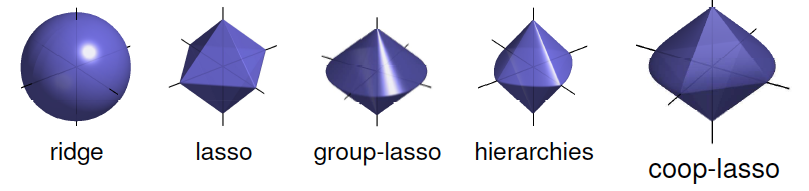
\includegraphics[scale=0.5]{group_sparse.png}
\end{center}
On considère $\{ \mathcal{G}_{k = 1}^K \}$ une partition de $\{ 1, \dots, d \}$. On peur alors définir les normes suivantes :
$$ \| \theta \|_{group} = \sum_{g \in \mathcal{G}} \left( \sum_{j \in g} \theta_j^2 \right)^{\frac{1}{2}} $$
$$ \| \theta \|_{coop} = \sum_{g \in \mathcal{G}} \left[ \left( \sum_{j \in g} [\theta_j]_+^2 \right)^{\frac{1}{2}} + \left( \sum_{j \in g} [\theta_j]_-^2 \right)^{\frac{1}{2}} \right] $$


\subs{Contrepartie Biais/Variance}

D'où vient l'erreur de $h \in \Hyp$ ?
\begin{itemize}
	\item Du \textbf{biais inductif}. Rien ne garantie l'égalité entre l'espace cible des concepts $\mathcal{F}$ et la classe d'hypothèse que l'on a choisi $\Hyp$.
	\item De la \textbf{variance}. Comme l'ensemble d'entraînement est fini et choisi aléatoirement selon $\dist$, l'algorithme d'apprentissage ne retourne pas l'hypothèse optimale $h^*$ de $\Hyp$.
\end{itemize}

\begin{center}
	\begin{tikzpicture}[thick]
		\draw (0, 0.5) -- (4, 0.5) -- (4, 2) -- node[above] {$\Hyp$} (0, 2) -- (0, 0.5);
		\node at (5.5, 0.5) {$\mathcal{F}$};
		\draw[fill] (0.5, 1) circle (0.05) node[above] {$h$}
			-- node[below, sloped] {\footnotesize erreur totale} (3.7, -1)
				circle (0.05) node[right] {$f$}
			-- node[above, sloped] {\footnotesize biais} (2.5, 1)
				circle (0.05) node[above] {$h^*$}
			-- node[above] {\footnotesize Variance} (0.5, 1);
	\end{tikzpicture}
\end{center}
$$ \trisk(h) \leqslant \text{Biais} + \text{Variance} $$
$$ \trisk(h) \leqslant \text{Biais inévitable} + \text{Biais évitable} + \text{Variance} $$
$$ \trisk(h) \leqslant {\color{red}\text{Erreur de Bayes}} + {\color{blue}\text{Biais évitable}} + {\color{blue}\text{Variance}} $$

\DEF{
	L'\textbf{erreur de Bayes} $\epsilon_B$ est le plus petit taux d'erreur pour une hypothèse $h$ :
	$$ \epsilon_B = \sum_i \int_{(x, y) \in R_i \times \bar{C_i}} P(C_i | x) p(x) dx $$
	Où $x$ est une instance avec $y$ pour étiquette et $R_i$ est la région que la fonction de classification $h$ classifie comme $C_i$.
}
\begin{center}
	C'est un $\ll$ sept $\gg$ ou un $\ll$ un $\gg$ ? \\
	
\includegraphics[scale=0.4]{one_seven.png}
\end{center}

\paragraph{Variance}
$h$ va converger vers $h^*$ si on augmente le nombre d'exemples $m$.
\begin{center}
	\begin{tikzpicture}[thick, scale=0.9]
		\draw[ultra thick, blue, opacity=0.8] (0, -2.5) -- (0, 2.5);
		\draw[ultra thick, blue, opacity=0.8] (-1.6, -2.5) -- (0.25, 2.5);
		\node[below] at (-1.6, -2.5) {$h$};
		\node[below] at (0, -2.5) {$h^*$};
		\draw[<->, red] (-0.3, -2.8) -- node[black, above] {?} (-1.4, -2.8);
		\draw[fill, red] (0.1, -2) circle (0.07);
		\draw[fill, red] (-0.6, -1) circle (0.07);
		\draw[fill, red] (0.3, 0.5) circle (0.07);
		\draw[fill, red] (0.5, 2) circle (0.07);
		\draw[fill, red, opacity=0.3] (-0.5, 0) circle (0.07);
		\draw[fill, red, opacity=0.3] (0.3243, 0.9859) circle (0.07);
		\draw[fill, red, opacity=0.3] (-0.08914, 0.978) circle (0.07);
		\draw[fill, red, opacity=0.3] (2.427, 0.7918) circle (0.07);
		\draw[fill, red, opacity=0.3] (1.4609, 1.212) circle (0.07);
		\draw[fill, red, opacity=0.3] (1.3548, 0.6159) circle (0.07);
		\draw[fill, red, opacity=0.3] (1.403, 0.351) circle (0.07);
		\draw[fill, red, opacity=0.3] (-0.351, 1.57183) circle (0.07);
		\draw[fill, red, opacity=0.3] (0.10869, 1.876) circle (0.07);
		\draw[fill, red, opacity=0.3] (-0.13232, 1.62) circle (0.07);
		\draw[fill, red, opacity=0.3] (0.048154, 0.0303) circle (0.07);
		\draw[fill, red, opacity=0.3] (0.0214, -0.861) circle (0.07);
		\draw[fill, red, opacity=0.3] (-0.10329, -1.902) circle (0.07);
		\draw[fill, red, opacity=0.3] (-0.049, -0.0497) circle (0.07);
		\draw[fill, red, opacity=0.3] (1.3507, -1.7576) circle (0.07);
		\draw[fill, red, opacity=0.3] (-0.4912, -0.3749) circle (0.07);
		\draw[fill, red, opacity=0.3] (1.0138, -0.184) circle (0.07);
		\draw[fill, red, opacity=0.3] (2.0108, 0.5766) circle (0.07);
		\draw[fill, red, opacity=0.3] (2.0224, 1.0361) circle (0.07);
		\draw[fill, red, opacity=0.3] (0.0751, 1.7442) circle (0.07);
		\draw[fill, red, opacity=0.3] (2.0863, 1.7777) circle (0.07);
		\draw[fill, red, opacity=0.3] (-0.0409, -0.1897) circle (0.07);
		\draw[fill, red, opacity=0.3] (0.2889, -0.0546) circle (0.07);
		\draw[fill, red, opacity=0.3] (2.4079, -0.1523) circle (0.07);
		\draw[fill, red, opacity=0.3] (1.8439, 1.2179) circle (0.07);
		
		\draw[fill, blue] (-0.8, 1.5) circle (0.07);
		\draw[fill, blue] (-1.2, 0.9) circle (0.07);
		\draw[fill, blue] (-1.6, -0.8) circle (0.07);
		\draw[fill, blue] (-1.6, -1.7) circle (0.07);
		\draw[fill, blue, opacity=0.3] (-1.9025, 0.0568) circle (0.07);
		\draw[fill, blue, opacity=0.3] (-0.2239, -0.3909) circle (0.07);
		\draw[fill, blue, opacity=0.3] (-0.6662, 0.0906) circle (0.07);
		\draw[fill, blue, opacity=0.3] (0.4667, 0.1391) circle (0.07);
		\draw[fill, blue, opacity=0.3] (-0.0517, -1.9698) circle (0.07);
		\draw[fill, blue, opacity=0.3] (-1.1208, -0.8846) circle (0.07);
		\draw[fill, blue, opacity=0.3] (0.1495, -0.2879) circle (0.07);
		\draw[fill, blue, opacity=0.3] (-2.4247, 0.4716) circle (0.07);
		\draw[fill, blue, opacity=0.3] (-1.9027, -1.2081) circle (0.07);
		\draw[fill, blue, opacity=0.3] (-1.4246, 1.5652) circle (0.07);
		\draw[fill, blue, opacity=0.3] (-1.729, 1.9974) circle (0.07);
		\draw[fill, blue, opacity=0.3] (-0.5392, 1.2422) circle (0.07);
		\draw[fill, blue, opacity=0.3] (0.3168, 0.8305) circle (0.07);
		\draw[fill, blue, opacity=0.3] (-0.2799, 0.1071) circle (0.07);
		\draw[fill, blue, opacity=0.3] (-1.5449, 0.0752) circle (0.07);
		\draw[fill, blue, opacity=0.3] (-1.8949, -0.0877) circle (0.07);
		\draw[fill, blue, opacity=0.3] (-0.9253, -0.423) circle (0.07);
		\draw[fill, blue, opacity=0.3] (0.279, -1.1842) circle (0.07);
		\draw[fill, blue, opacity=0.3] (-0.152, 0.5651) circle (0.07);
		\draw[fill, blue, opacity=0.3] (-0.8953, -1.1821) circle (0.07);
		\draw[fill, blue, opacity=0.3] (-0.3335, 1.352) circle (0.07);
		\draw[fill, blue, opacity=0.3] (-0.4852, -1.6634) circle (0.07);
	\end{tikzpicture}
\end{center}

\paragraph{Biais évitable}
La distance entre l'espace $\Hyp$ et $f$ va diminuer si on augmente l'expressivité de $h$ et notamment en augmentant la dimension.

\paragraph{Conclusion}
Malheureusement, augmenter la dimension augmente aussi la variance. Il faut donc trouver un bon compromis sur la dimension pour réduire le biais sans trop augmenter la variance.
\begin{center}
	\begin{tikzpicture}[thick, >={latex}]
		\draw[->] (0, 0) -- (5, 0) node[below] {dimension de $\Hyp$};
		\draw[->] (0, 0) -- (0, 3.5);
		\draw[domain=0:4.2, smooth, variable=\x, blue]
			plot ({\x}, {3 - \x * (0.33 + 0.05 * \x)})
			node[right] {\footnotesize Biais};
		\draw[domain=0:4.2, smooth, variable=\x, blue]
			plot ({\x}, {0.1 + 0.08 * \x + 0.42 * exp(1.44 * \x - 4.2)})
			node[right] {\footnotesize Variance};
		\draw[domain=0:4, smooth, variable=\x, red]
			plot ({\x}, {3.1 - \x * (0.25 + 0.05 * \x) + 0.42 * exp(1.44 * \x - 4.2)});
		\draw[red] (2.85, 0.3) -- (2.85, 2.7) node[above] {\footnotesize $\trisk(h)^{min}$};
	\end{tikzpicture}
\end{center} 

\subs{Bornes de généralisation}

\paragraph{But}
Notre objectif est d'obtenir des bornes \textbf{PAC (Probably Approximately Correct)} de la forme suivante : Avec probabilité $1 - \delta$
$$ \begin{array}{lll}
	\trisk(h) & \leqslant & \erisk(h) + \gamma \\
	 & \leqslant & \erisk(h^*) + 2 \gamma \qquad \text{(car } h = \argmin_{h_i \in \Hyp} \erisk(h_i)) \\
	 & \leqslant & (\trisk(h^*) + \gamma) + \gamma \\
	 & \leqslant & \trisk(h^*) + 2 \gamma
\end{array} $$

La théorie de la convergence uniforme nous donne des garanties pour les hypothèses $h \in \Hyp$. La question que l'on se pose est : Sous quelle conditions (sur le nombre minimum d'exemples d'entraînement requis) peut-on obtenir des bornes PAC valides ? \\
On va considérer deux situations. La première est celle où $|\Hyp| = k$ est fini. La seconde est celle où $\Hyp$ est infini.

\subsubs{Convergence uniforme - Cas fini}

On commence par rappeler le lemme suivant: \vspace{3mm}
\PROP[ (Inégalité de Hoeffding)]{
	Soit $Z_1, \dots, Z_m$ $m$ variables i.i.d suivant des loi de Bernoulli d'espérance $\phi$. On pose la variable $\hat{\phi} = \frac{1}{m} \sum_{i = 1}^m Z_i$ et on considère $\gamma > 0$. Alors : \vspace{-2mm}
	$$ \Pp(|\hat{\phi} - \phi| > \gamma) \leqslant 2 \exp(-2 \gamma^2 m) $$
	\vspace{-9mm}
}
\vspace{2mm}

On considère alors l'espace $\Hyp = \{ h_1, \dots, h_k \}$. L'inégalité de Hoeffding peut être appliqué à $\trisk(h)$ et $\erisk(h)$ avec $l(h, z_i)$ qui est une loi de Bernoulli d'espérance $\trisk(h)$. On pose donc $A_j$ l'événement $| \trisk(h) - \erisk(h) | \geqslant \gamma$. Avec l'inégalité de Hoeffding, on a : $\Pp(A_j) \leqslant 2 e^{-2 \gamma^2 m}$. Et cela donne :
$$ \begin{array}{lll}
	\Pp(\sup_{h \in \Hyp} | \trisk(h) - \erisk(h) | \geqslant \gamma )
	 & = & \Pp(A_1 \cup \dots \cup A_k) \\
	 & \leqslant & \sum_j \Pp(A_j) \\
	 & \leqslant & \sum_j 2 e^{-2 \gamma^2 m} \\
	 & \leqslant & 2k e^{-2 \gamma^2 m}
\end{array} $$

\paragraph{Borne sur $m$}
Avec l'inégalité précédente on peut essayer de trouver la valeur minimale de $m$ pour que la probabilité soit au plus $\delta$ :
$$ \begin{array}{lll}
	2k e^{-2 \gamma^2 m} \leqslant \delta
	 & \Leftrightarrow & e^{2 \gamma^2 m} \geqslant \dfrac{2k}{\delta} \\
	 & \Leftrightarrow & 2 \gamma^2 m \geqslant \ln \left( \dfrac{2k}{\delta} \right) \\
	 & \Leftrightarrow & m \geqslant \dfrac{1}{2 \gamma^2} \ln \left( \dfrac{2k}{\delta} \right)
\end{array} $$
Donc si $m \geqslant \dfrac{1}{2 \gamma^2} \ln \left( \dfrac{2k}{\delta} \right)$ alors avec probabilité $1 - \delta$, on a :
$$ \trisk(h) \leqslant \erisk(h) + \gamma $$
Mais généralement $m$ est fixé.

\paragraph{Borne sur $\gamma$}
Pour un $m$ fixé et une probabilité $\delta$ fixée, on obtient :
$$ \gamma = \sqrt{\dfrac{1}{2m} \ln \left( \dfrac{2k}{\delta} \right)} $$

\PROP[ (Borne de généralisation dans le cas fini)] {
	Avec probabilité $1 - \delta$, on a pour tout $h$ dans $\Hyp$ :
	$$ \trisk(h) \leqslant \erisk(h) + \sqrt{\dfrac{1}{2m} \ln \left( \dfrac{2k}{\delta} \right)} $$
	\vspace{-5mm}
}

\subsubs{Convergence uniforme - Cas infini}

On introduit la dimension VC (pour Vapnik-Chervonenkis) qui est une mesure de la capacité (ou complexité) de la classe des hypothèses $\Hyp$.

\DEF{
	Un ensemble de point $S$ est \textbf{pulvérisé} par $\Hyp$ si pour tout sous-ensembles $A$ de $S$, il existe une hypothèse $h \in \Hyp$ qui ne fait pas d'erreur sur $A$. Autrement dit $S$ est pulvérisé par $\Hyp$ si les éléments de $\Hyp$ permettent d'obtenir les $2^{|S|}$ dichotomies de $S$. \\
	La \textbf{dimension VC} $d_\Hyp$ d'une classe d'hypothèses $\Hyp$ est défini comme le plus grand cardinal de points que $\Hyp$ peut pulvériser.
}

\begin{center}
	\begin{tikzpicture}[thick, >={latex}]
		\draw (0, 5.5) circle (0.12);
		\draw (1, 5.5) circle (0.12);
		\draw (1, 4.5) circle (0.12);
		\draw (4, 5.5) circle (0.12);
		\draw (10, 5.5) circle (0.12);
		\draw (10, 4.5) circle (0.12);
		\draw (1, 2.5) circle (0.12);
		\draw (3, 3.5) circle (0.12);
		\draw (6, 3.5) circle (0.12);
		\draw (7, 3.5) circle (0.12);
		\draw (9, 3.5) circle (0.12);
		\draw (10, 2.5) circle (0.12);
		
		\draw[fill] (3, 5.5) circle (0.12);
		\draw[fill] (4, 4.5) circle (0.12);
		\draw[fill] (6, 5.5) circle (0.12);
		\draw[fill] (7, 5.5) circle (0.12);
		\draw[fill] (7, 4.5) circle (0.12);
		\draw[fill] (9, 5.5) circle (0.12);
		\draw[fill] (0, 3.5) circle (0.12);
		\draw[fill] (1, 3.5) circle (0.12);
		\draw[fill] (4, 3.5) circle (0.12);
		\draw[fill] (4, 2.5) circle (0.12);
		\draw[fill] (7, 2.5) circle (0.12);
		\draw[fill] (10, 3.5) circle (0.12);
		
		\draw (-1, 4) -- (11, 4);
		\draw (2, 2.2) -- (2, 5.8);
		\draw (5, 2.2) -- (5, 5.8);
		\draw (8, 2.2) -- (8, 5.8);
		
		\draw (-0.5, 5.7) -- (1.2, 4);
		\draw[->] (0.35, 4.85) -- (0.05, 4.55);
		\draw (3.3, 5.7) -- (4.2, 4.8);
		\draw[->] (3.75, 5.25) -- (3.45, 4.95);
		\draw (5.5, 5.7) -- (7.2, 4);
		\draw[->] (6.35, 4.85) -- (6.65, 5.15);
		\draw (9.5, 4.2) -- (9.5, 5.7);
		\draw[->] (9.5, 5) -- (9.05, 5);
		\draw (-0.3, 3) -- (1.3, 3); 
		\draw[->] (0.5, 3) -- (0.5, 3.45);
		\draw (3.5, 2.2) -- (3.5, 3.8);
		\draw[->] (3.5, 3) -- (3.95, 3);
		\draw (5.7, 3) -- (7.3, 3); 
		\draw[->] (6.5, 3) -- (6.5, 2.55);
		\draw (9.2, 3.7) -- (10.2, 2.7);
		\draw[->] (9.7, 3.2) -- (9.9, 3.4);
	\end{tikzpicture}
\end{center}

Avec $d_\Hyp$ on peut obtenir une borne pour $\trisk(h)$.

\PROP[ (Borne de généralisation dans le cas infini)] {
	Avec probabilité $1 - \delta$, on a pour tout $h$ dans $\Hyp$ :
	$$ \trisk(h) \leqslant \erisk(h) + \sqrt{\dfrac{d_\Hyp \left( \ln \frac{2 m}{d_\Hyp} + 1 \right) + ln \frac{4}{\delta}}{m}} $$
	\vspace{-5mm}
}

Au lieu d'utiliser la dimension VC, on peut aussi utiliser la complexité de Rademacher.

\DEF{
	La \textbf{complexité empirique de Rademacher} de $\Hyp$ est :
	$$ Rad_m(\Hyp, S) = \E \left( \sup_{h \in \Hyp} \left| \frac{1}{m} \sum_{i = 1}^m \sigma_i h(z_i) \right| \right) $$
	Où $\sigma_1, \dots, \sigma_m$ sont $m$ variables de Rademacher i.i.d avec $\Pp(\sigma_i = 1) = \Pp(\sigma_i = -1) = \frac{1}{2}$.
}

\PROP[ (Borne de convergence uniforme avec la complexité de Rademacher)] {
	Avec probabilité $1 - \delta$, on a pour tout $h$ dans $\Hyp$ : \vspace{-3mm}
	$$ \trisk(h) \leqslant \erisk(h) + 2 Rad_m(\Hyp, S) + \sqrt{\dfrac{4}{m} ln \left( \dfrac{2}{\delta} \right)} $$
	\vspace{-5mm}
}

\subs{Choix du modèle}
	\chapter{Régression Linéaire/Polynomiale/Logistique}

\myminitoc

SOON !!!

\sect{Introduction}

On va considérer des modèles $h$ sous forme linéaire.
$$ h_\theta(x) = \sum_{i = 0}^n \theta_i x_i = \theta^\trans x $$
On posera toujours $x_0 = 1$ pour avoir une ordonnée à l'origine. Le but sera alors de trouver $\theta \in \R^{n+1}$ pour que $h$ fasse des prédictions précises.

\begin{center}
	\begin{tikzpicture}[thick, >={latex}]
		\draw[->, blue] (0, 0) -- (6, 0);
		\draw[->, blue] (0, 0) -- (0, 4);
		\draw[fill] (0.357143, 0.395123) circle (0.10);
		\draw[fill] (1.146921, 1.641947) circle (0.10);
		\draw[fill] (1.740568, 1.906676) circle (0.10);
		\draw[fill] (1.835173, 1.007108) circle (0.10);
		\draw[fill] (2.915078, 2.585541) circle (0.10);
		\draw[fill] (3.815745, 2.650688) circle (0.10);
		\draw[fill] (4.439558, 2.812134) circle (0.10);
		\draw[domain=0:5.000000, smooth, variable=\x, red] 
			plot ({\x}, {0.568668 + \x * 0.554981});
		\draw [decorate, decoration={brace,amplitude=2pt}, xshift=-0.1cm, greenTikz]
			(0, 0) -- node [left] {$\theta_0$} (0, 0.568);
		\draw[dashed] (1.835, 1) -- (1.835, 1.59);
		\draw [decorate, decoration={brace,amplitude=2pt}, xshift=0.2cm, greenTikz]
			(1.835, 1.59) -- node [right] {$h_\theta(x) - y$} (1.835, 1);
	\end{tikzpicture}
\end{center}

On se posera alors le \textbf{problème des moindres carrées} :
$$ \min_\theta J(\theta) = \min_\theta \dfrac{1}{2m} \sum_{i = 1}^m \left( h_\theta(x^{(i)}) - y^{(i)} \right)^2 $$
Il y a plusieurs méthodes pour minimiser $J(\theta)$ :
\begin{itemize}
	\item \textbf{Descente de gradient par batchs}
	\item \textbf{Descente de gradient stochastique}
	\item \textbf{Descente de gradient par mini-batchs}
	\item \textbf{Solution de forme fermée}
\end{itemize}

\sect{Régression linéaire et polynomiale}

\subs{Descente de gradient}

\subsubs{Descente de gradient par batchs}

\paragraph{Idée basique}
Si $J(\theta)$ est différentiable, l'idée est la suivante :
\begin{itemize}
	\item Initialiser $\theta$ avec la valeur 0 ou par un vecteur aléatoire.
	\item Mettre à jour $\theta$ de manière à réduire $J(\theta)$ après avoir calculer les dérivées partielles de $J(\theta)$.
	\item Puis répéter ce processus jusqu'à convergence vers un minimum de $J(\theta)$.
\end{itemize}
La formule de mise à jour de $\theta$ est la suivant :
$$ \theta_i \gets \theta_i - \alpha \dfrac{\partial}{\partial \theta_i} J(\theta) $$
Où $\alpha$ est une constante qui s'appelle le \textbf{taux d'apprentissage} et qui permet de contrôler la grandeur des pas que l'on fait. \\
En utilisant la notation du gradient : $ \nabla_\theta J = \begin{bmatrix}
\frac{\partial}{\partial \theta_0} \\ \vdots \\ \frac{\partial}{\partial \theta_n}
\end{bmatrix} $, on peut réécrire la mise à jour comme cela :
\begin{center}
	\boldmath \fbox{$ \displaystyle \theta \gets \theta - \alpha \nabla_\theta J$}
\end{center}

\paragraph{Mise à jour du $i$-ème paramètre}
On se place dans le cas où $m = 1$. C'est à dire :
$$ J(\theta) = \dfrac{1}{2} (h_\theta(x) - y)^2 $$
On calcule alors la dérivée partielle selon $\theta_i$ :
$$ \begin{array}{lll}
	\dfrac{\partial}{\partial \theta_i} J(\theta)
	& = & \dfrac{\partial}{\partial \theta_i} \dfrac{1}{2} (h_\theta(x) - y)^2 \\
	& = & 2 \times \dfrac{1}{2} (h_\theta(x) - y) \times \dfrac{\partial}{\partial \theta_i}  (h_\theta(x) - y) \\
	& = & (h_\theta(x) - y) \times \dfrac{\partial}{\partial \theta_i}  (\theta_0 x_0 + ... + \theta_i x_i + ... + \theta_n x_n - y) \\
	& = & (h_\theta(x) - y) x_i
\end{array} $$
Ce qui nous permet d'avoir : $ \theta_i \gets \theta_i - \alpha (h_\theta(x) - y) x_i $. \\
Dans le cas générale on obtient alors :
\begin{center}
	\boldmath \fbox{$ \displaystyle \theta_i \gets \theta_i - \alpha \dfrac{1}{m} \sum_{j = 1}^m \left( h_\theta(x^{(j)}) - y^{(j)} \right) x_i^{(j)}$}
\end{center}
A noter qu'on parle de batch car à chaque descente de gradient on regarde l'ensemble d'entraînement en entier.

\REM{
	Avec des initialisation légèrement différentes, on peut converger vers des minimums locaux complètement différents
	\begin{center}
		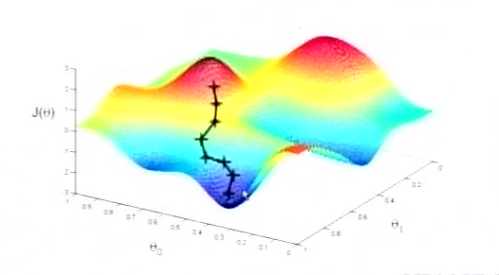
\includegraphics[scale=1.6]{grad1.png}
		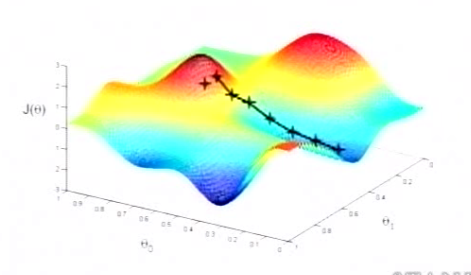
\includegraphics[scale=1.6]{grad2.png}
	\end{center}
}

\paragraph{Choix de $\alpha$}
Il est important de bien choisir $\alpha$, car si sa valeur est trop élevé il est possible que $J(\theta)$ croisse. Une valeur faible de $\alpha$ est donc préférable mais il faut savoir que plus sa valeur est faible, plus le temps de convergence sera long ...
\begin{center}
	\begin{tikzpicture}[thick, >={latex}, scale=0.9]
		\draw[domain=1.181978:6.956124, smooth, variable=\x, blue] 
			plot ({\x}, {0.5 * (\x - 4)^2});
		\draw[->, greenTikz]
			(2.000000, 2.000000) -- node[right] {\footnotesize petit $\alpha$} (3.500000, 0.125000);
		\draw[->, red]
			(2.000000, 2.000000) -- node[below] {\footnotesize grand $\alpha$} (6.160000, 2.332800);
		\draw[->, greenTikz] (3.500000, 0.125000) -- (3.875000, 0.007812);
		\draw[->, red] (6.160000, 2.332800) -- (1.667200, 2.720978);
		\draw[->, greenTikz] (3.875000, 0.007812) -- (3.968750, 0.000488);
		\draw[->, red] (1.667200, 2.720978) -- (6.519424, 3.173749);
		\draw[fill] (2, 2) circle (0.1);
	\end{tikzpicture}
\end{center}

\paragraph{Pour}
\begin{itemize}
	\item Peu de mises à jour sont nécessaires car le gradient est stable.
	\item La séparation en somme de la mise à jour permet d'utiliser des algorithmes parallèles
\end{itemize}
\paragraph{Contre}
\begin{itemize}
	\item La stabilité du gradient peu conduire prématurément vers un minimum local pas très optimal.
	\item La mise à jour peut prendre beaucoup de temps pour de grandes bases de données.
\end{itemize}

\subsubs{Descente de gradient stochastique}

Si la base de donnée est grande, disons 1 million d'exemples alors à chaque itération de le descente de gradient par batchs, on doit réaliser une somme d'erreurs sur un million d'exemples. Pour plus de rapidité il nous faut donc penser à un autre algorithme où l'on fait des mises à jour de $\theta$ plus régulièrement :

\begin{center}
	\begin{algorithm}[H]
		Initialisation de $\theta$\;
		\Repeat{convergence de $J(\theta)$}{
			\For{$j=1$ à $m$}{
				$\forall i, \; \theta_i \gets \theta_i - \alpha \left( h_\theta(x^{(j)}) - y^{(j)} \right) x_i^{(j)} $
			}
		}
		\caption{Descente de gradient stochastique}
	\end{algorithm}
\end{center}

\paragraph{Pour}
\begin{itemize}
	\item La fréquence élevé des mises à jour qui peut donner un apprentissage plus rapide.
	\item Ces mise à jours un peu "chaotiques" et instables peuvent empêcher de converger vers des minimas locaux.
	\item Cet algorithme permet aussi d'avoir un acquisition de données en ligne.
\end{itemize}
\paragraph{Contre}
L'algorithme ne converge pas vers le minimum globale mais il a tendance à rester autour.

\paragraph{Descente de gradient par mini-batchs}
Pour gagner en robustesse et garder l'efficacité de la descente stochastique, on peut séparer l'ensemble d'entraînement en de petits sous-ensembles (des petits batchs). Puis on reprend la descente stochastique mais au lieu de mettre à jour $\theta$ en s'appuyant sur un seul exemple à la fois, on le met à jour en fonction de l'erreur sur un mini-batch.

\subs{Solution de forme fermée}

On pose les vecteurs et matrices suivantes :
$$ x^{(j)} = \begin{pmatrix} x_0^{(j)} \\ \vdots \\ x_n^{(j)} \end{pmatrix} \qquad
X = \begin{pmatrix} {x^{(1)}}^\trans \\ \vdots \\ {x^{(m)}}^\trans \end{pmatrix} \qquad 
\theta = \begin{pmatrix} \theta_0 \\ \vdots \\ \theta_n \end{pmatrix} \qquad
y = \begin{pmatrix} y^{(1)} \\ \vdots \\ y^{(m)} \end{pmatrix} $$
Cela nous permet de réécrire $J(\theta)$.
$$ J(\theta) = \dfrac{1}{2m} (X\theta - y)^\trans (X\theta - y) $$
En un minimum de $J$, le gradient est nul. On cherche donc à résoudre :
$$ \nabla_\theta \dfrac{1}{2} (X\theta - y)^\trans (X\theta - y) = 0 $$
\newpage

$$ \begin{array}{lll}
\nabla_\theta \dfrac{1}{2} (X\theta - y)^\trans (X\theta - y)
& = & \dfrac{1}{2} \nabla_\theta \left( \theta^\trans X^\trans X \theta - \theta^\trans X^\trans y - y^\trans X \theta + y^\trans y \right) \\ \\
& = & \dfrac{1}{2} \left[ \nabla_\theta \left(\theta^\trans X^\trans X \theta \right) - 2 \nabla_\theta \left( y^\trans X \theta \right) \right] \\ \\
& = & X^\trans X \theta - X^\trans y
\end{array} $$

\PROP[ (Solution de forme fermée)]{
	Ainsi, si $X^\trans X$ est inversible, l'expression de $\theta$ suivante est optimale :
	\vspace{-1mm}
	$$\theta = (X^\trans X)^{-1} X^\trans y$$
	En revanche si $X^\trans X$ n'est pas inversible, il est possible que des features soient redondants. Appliqué l'algorithme PCA peut alors être une solution.
}

\subs{Régression polynomiale}

Dans le cas d'une régression polynomiale, on $h_\theta(x) = \theta_0 + \theta_1 x + \theta_2 x^2 + ... + \theta_n x^n$. La fonction est toujours linéaire selon $\theta$. L'idée est alors de se placer en dimension $n+1$, en posant $x_i = x^i$.

\sect{Interprétation probabiliste de la régression}

On peut se poser la question : Pourquoi les moindres carrées ? Pourquoi ne pas minimiser la valeur absolue ou encore la puissance 4 ?

Supposons que l'erreur sur $y^{(i)}$ suit une loi gaussienne. Ceci est justifié par le théorème centrale limite. On a donc :
$$ y^{(i)} = \theta^\trans x^{(i)} + \epsilon^{(i)} $$
Où $\epsilon^{(i)} \sim \mathcal{N}(0, \sigma)$. \\
On va ensuite chercher à maximiser la vraisemblance de $y$.

\DEF{
	Soit $X_1, ..., X_m$ des variables aléatoires i.i.d de densité $f(x|\theta)$ où $\theta$ est un paramètre de la loi. Pour un échantillon $X_1 = x_1, ..., X_n = x_n$ donné, la \textbf{vraisemblance} est : \vspace{-3mm}
	$$ L(\theta) = f(x_1, ..., x_n) = \prod_{i=1}^m f(x_i|\theta) $$
	\vspace{-7mm}
}

On a donc dans notre cas :
$$ L(\theta) = \Pp(y | X, \theta) = \prod_{i=1}^m \Pp(y^{(i)} | x^{(i)}, \theta) = \prod_{i=1}^m \dfrac{1}{\sqrt{2 \pi} \sigma} \exp \left( - \dfrac{(y^{(i)} - \theta^\trans x^{(i)})^2}{2 \sigma^2} \right) $$
Une bonne manière d'étudier la vraisemblance est de la passer au logarithme car elle est souvent log-concave. La log-vraisemblance est notée $l(\theta) = \ln L(\theta)$. Voici alors ce qu'on obtient si on simplifie l'expression de la log-vraisemblance :

$$ \begin{array}{lll}
	l(\theta)
	& = & \displaystyle \sum_{i = 1}^m \ln \left( \dfrac{1}{\sqrt{2 \pi} \sigma} \exp \left( - \dfrac{(y^{(i)} - \theta^\trans x^{(i)})^2}{2 \sigma^2} \right) \right) \\
	& = & \displaystyle \sum_{i = 1}^m \ln \dfrac{1}{\sqrt{2 \pi} \sigma} + \sum_{i = 1}^m \left( - \dfrac{(y^{(i)} - \theta^\trans x^{(i)})^2}{2 \sigma^2} \right) \\
	& = & \displaystyle m \ln \dfrac{1}{\sqrt{2 \pi} \sigma} - \sum_{i = 1}^m \dfrac{(y^{(i)} - \theta^\trans x^{(i)})^2}{2 \sigma^2}
\end{array} $$
Ainsi maximiser $l(\theta)$ revient à minimiser $\displaystyle J(\theta) = \sum_{i = 1}^m \dfrac{(y^{(i)} - \theta^\trans x^{(i)})^2}{2}$ \\
Donc lorsque l'on utilise l'algorithme des moindres carrées, on maximise simplement la vraisemblance en assumant que les erreurs sur les $y^{(i)}$ sont i.i.d selon une loi normale.

\sect{Régression régularisée}

Comme on l'a vu à la fin du chapitre précédent, il y a des risques d'overfitting. Une solution est la régularisation. On parle de régularisation \textbf{ridge} pour la norme $l_2$ et de régularisation \textbf{LASSO} pour la norme $l_1$.

\begin{center}
	\begin{tikzpicture}[thick, >={latex}]
	\draw[domain=0:360, smooth, variable=\t, very thick, fill=greenTikz, fill opacity=0.6]
	plot ({1.800000 + 3.035357 * cos(\t) + 0.443197 * sin(\t)}, {1.700000 + -1.107992 * cos(\t) + 1.214143 * sin(\t)});
	\draw[domain=0:360, smooth, variable=\t, very thick] 
	plot ({1.800000 + 0.758839 * cos(\t) + 0.110799 * sin(\t)}, {1.700000 + -0.276998 * cos(\t) + 0.303536 * sin(\t)});
	\draw[domain=0:360, smooth, variable=\t, very thick] 
	plot ({1.800000 + 1.517678 * cos(\t) + 0.221598 * sin(\t)}, {1.700000 + -0.553996 * cos(\t) + 0.607071 * sin(\t)});
	\draw[domain=0:360, smooth, variable=\t, very thick] 
	plot ({1.800000 + 2.276518 * cos(\t) + 0.332398 * sin(\t)}, {1.700000 + -0.830994 * cos(\t) + 0.910607 * sin(\t)});
	
	\draw[domain=0:360, smooth, variable=\t, very thick, fill=greenTikz, fill opacity=0.6]
	plot ({10.800000 + 3.289353 * cos(\t) + 0.480283 * sin(\t)}, {1.700000 + -1.200708 * cos(\t) + 1.315741 * sin(\t)});
	\draw[domain=0:360, smooth, variable=\t, very thick] 
	plot ({10.800000 + 0.822338 * cos(\t) + 0.120071 * sin(\t)}, {1.700000 + -0.300177 * cos(\t) + 0.328935 * sin(\t)});
	\draw[domain=0:360, smooth, variable=\t, very thick] 
	plot ({10.800000 + 1.644677 * cos(\t) + 0.240142 * sin(\t)}, {1.700000 + -0.600354 * cos(\t) + 0.657871 * sin(\t)});
	\draw[domain=0:360, smooth, variable=\t, very thick] 
	plot ({10.800000 + 2.467015 * cos(\t) + 0.360212 * sin(\t)}, {1.700000 + -0.900531 * cos(\t) + 0.986806 * sin(\t)});
	
	\draw[->] (0, -1.5) -- (0, 3.8);
	\draw[->] (-2, 0) -- (5, 0);
	\draw[->] (9, -1.5) -- (9, 3.8);
	\draw[->] (7, 0) -- (14, 0);
	\draw[very thick, fill=purple] (0, 0) circle (1);
	\draw[very thick, fill=purple] (9, 1) -- (8, 0) -- (9, -1) -- (10, 0) -- cycle;
	\fill[redLight] (9, 1) circle (0.16);
	\fill[redLight] (0.342898, 0.939373) circle (0.16);
	\node[red] at (4, 3.5) {Ridge};
	\node[red] at (13, 3.5) {LASSO};
	\end{tikzpicture}
\end{center}

\PROP[ (Forme fermée pour Ridge)]{
	Pour le régression ridge, la solution de forme fermée est la suivante :
	$$\theta = (X^\trans X + \lambda I_{n+1})^{-1} X^\trans y $$
	\vspace{-8mm}
}

\PROP[ (Stabilité uniforme pour Ridge)]{
	Avec la régression ridge, on obtient la borne de généralisation suivante :
	$$ \trisk(h_\theta) \leqslant \erisk(h_\theta) + \dfrac{4 B^2}{\lambda m} + \left( \dfrac{8 B^2}{\lambda} + 2B \right) \sqrt{\dfrac{\ln 1/\delta}{2m}} $$
	Où $\Y$ est bornée et $\Y = [0, B]$.
}

En revanche pour la régularisation LASSO, on ne dispose pas de résultats précis, mais on sait que l'utilisation de cette régularisation conduit à une diminution du nombre de paramètres non nuls. Ainsi LASSO permet d'avoir le vecteur $\bm{\theta}$ \textbf{creux}.

\sect{Machine à vecteur de support (SVR)}

Jusque là nous utilisé la méthode des moindres carrés. Il y a aussi la \textbf{perte $\bm{\epsilon}$-sensible} :
$$ \min_{\theta, \xi, \xi^*} \frac{1}{2} \| \theta \|_2^2 + C \sum_{i = 1}^m \left( \xi_i + \xi_i^* \right) $$
\vspace{-2mm}
$$ \text{s.t. } \left\{ \begin{array}{l}
	y^{(i)} - \theta^\trans x^{(i)} \leqslant \epsilon + \xi_i \\
	\theta^\trans x^{(i)} - y^{(i)} \leqslant \epsilon + \xi_i^* \\
	\xi_i, \xi_i^* \geqslant 0
\end{array} \right. $$

Le lagrangien de ce problème est alors le suivant :
$$ L(\theta, \xi, \xi^*, \alpha, \alpha^*, \beta, \beta^*) = \dfrac{1}{2} \| \theta \|^2 + C \mathbbm{1}_m^\trans \left( \xi + \xi^* \right) + \alpha^\trans \left( y - X \theta - \epsilon \mathbbm{1}_m - \xi \right) + {\alpha^*}^\trans \left( X \theta - y - \epsilon \mathbbm{1}_m - \xi \right) - \beta^\trans \xi - {\beta^*}^\trans \xi^*$$
On rappelle que la fonction objective du dual est :
$$ g(\alpha, \alpha^*, \beta, \beta^*) = \inf_{\theta, \xi, \xi^*} L(\theta, \xi, \xi^*, \alpha, \alpha^*, \beta, \beta^*) $$
On cherche maintenant ce que vaut $\theta$ dans l'expression de $g$.
$$ \dfrac{\partial L}{\partial \theta} = \theta - X^\trans \alpha + X^\trans \alpha^* $$
$$ \dfrac{\partial L}{\partial \xi} = C \mathbbm{1}_m - \alpha - \alpha^* - \beta \qquad \qquad
\dfrac{\partial L}{\partial \xi^*} = C \mathbbm{1}_m - \alpha - \alpha^* - \beta^* $$
D'où $\theta = X^\trans (\alpha - \alpha*)$ et $\beta = \beta^* = C \mathbbm{1} - (\alpha + \alpha^*)$. On obtient alors :
$$ g(\alpha, \alpha^*) = -\dfrac{1}{2} (\alpha - \alpha^*)^\trans X X^\trans (\alpha - \alpha^*) + (\alpha - \alpha^*)^\trans y - \epsilon (\alpha + \alpha^*)^\trans \mathbbm{1}_m $$
Et on a la condition $\alpha + \alpha^* \leqslant C \mathbbm{1}_m$ car $\beta$ et $\beta^*$ sont positifs. \\ Soit alors $(\alpha, \alpha^*)$ une solution. Supposons $\alpha \geqslant \alpha^*$. On pose $\nu = \alpha - \alpha^*$. On a alors $\nu \leqslant \alpha + \alpha^*$ et $\nu - 0 = \alpha - \alpha^*$. Donc $(\nu, 0)$ est aussi une solution, et $g(\nu, 0) \geqslant g(\alpha, \alpha^*)$. \\
On obtient finalement le problème dual suivant :
\begin{center}
	\fbox{$ \displaystyle \min_{|\nu_i| \leqslant C} \dfrac{1}{2} \left\| X^\trans \nu \right\|_2^2 - \nu^\trans y + \epsilon \| \nu \|_1 $}
\end{center}
Dans ce cas, on a $\theta = X^\trans \nu$, et $h_\nu(x) = \theta^\trans x = \nu^\trans X x$.

\paragraph{Astuce du noyau}
Dans le cas non, linéaire il existe une astuce du noyau. Il est bon de le savoir mais je ne vais pas en parler ici.

\sect{De la régression à la classification}

\subs{Régression logistique}

Jusqu'à maintenant, nous avons considéré $y \in \R$. On se place désormais dans le cas où $y \in \{0, 1\}$. Par exemple $y = 1$ lorsque le patient a une maladie et $y = 0$ sinon. Dans ce cas c'est généralement une  mauvaise idée d'utiliser un régression linéaire.

\begin{center}
	\begin{tikzpicture}[scale=2, thick, >={latex}]
		\draw[->] (-0.2, 0) -- (2.3, 0);
		\draw[->] (0, -0.2) -- (0, 1.3);
		\draw[fill=blue] (0.2, 0) circle(0.04);
		\draw[fill=blue] (0.3, 0) circle(0.04);
		\draw[fill=blue] (0.4, 0) circle(0.04);
		\draw[fill=blue] (0.5, 0) circle(0.04);
		\draw[fill=blue] (0.6, 1) circle(0.04);
		\draw[fill=blue] (0.7, 1) circle(0.04);
		\draw[fill=blue] (0.8, 1) circle(0.04);
		\draw[fill=blue] (0.9, 1) circle(0.04);
		\draw[fill=blue] (2, 1) circle(0.04);
		\draw[domain=0:1.8, smooth, variable=\x, red] plot ({\x}, {0.107+0.631*\x});
	\end{tikzpicture}
\end{center}

On utilise alors la régression logistique.

\DEF{
	La fonction \textbf{sigmoïde (logistique)} est définie par :
	$$ sig(z) = \dfrac{1}{1 + e^{-z}} $$
	\vspace{-3mm}
	Et sa fonction réciproque, la fonction \textbf{logit} est définie par :
	$$ logit(p) = \ln \left( \dfrac{p}{1-p} \right) $$
	\vspace{-6mm}
}

Cette fonction nous permet de définir le nouveau modèle :
\begin{center}
	\boldmath \fbox{$ \displaystyle h_\theta(x) = g \left( \theta^\trans x \right) = \dfrac{1}{1 + e^{-\theta^\trans x}} $}
\end{center}

\begin{center}
	\begin{tikzpicture}[scale=2, thick, >={latex}]
	\draw[->] (-0.2, 0) -- (2.3, 0);
	\draw[->] (0, -0.2) -- (0, 1.3);
	\draw[fill=blue] (0.2, 0) circle(0.04);
	\draw[fill=blue] (0.3, 0) circle(0.04);
	\draw[fill=blue] (0.4, 0) circle(0.04);
	\draw[fill=blue] (0.5, 0) circle(0.04);
	\draw[fill=blue] (0.6, 1) circle(0.04);
	\draw[fill=blue] (0.7, 1) circle(0.04);
	\draw[fill=blue] (0.8, 1) circle(0.04);
	\draw[fill=blue] (0.9, 1) circle(0.04);
	\draw[fill=blue] (2, 1) circle(0.04);
	\draw[domain=0.3:2, smooth, variable=\x, greenTikz, ultra thick] plot ({\x}, {1 / (1 + exp(-30.1*\x+16.55))});
	\draw[ultra thick, greenTikz] (0, 0) -- (0.3, 0);
	\end{tikzpicture}
\end{center}

Ainsi si $\theta^\trans > 0$ alors $h_\theta(x) > \frac{1}{2}$ et on pose $\hat{y} = 1$ sinon on pose $\hat{y} = 0$. On peut voir $h_\theta(x)$ comme une probabilité tel que $\Pp(y = 1|x, \theta) = h_\theta(x)$. \\
La méthode des moindres carrées est adaptée pour la régression mais pour la classification on préfère maximiser la vraisemblance puisque $h_\theta$ représente une probabilité.
$$ \Pp(y = 1 | x, \theta) = h_\theta(x) \qquad \text{et} \qquad \Pp(y = 0 | x, \theta) = 1 - h_\theta(x) $$
Cela nous donne :
$$ \Pp(y | x, \theta) = h_\theta(x)^y \left( 1 - h_\theta(x) \right)^{1-y} $$
On en déduit ensuite la vraisemblance :
$$ L(\theta) = \prod_{i=1}^m \Pp(y^{(i)} | x^{(i)}, \theta) = \prod_{i=1}^m h_\theta(x^{(i)})^{y^{(i)}} \left( 1 - h_\theta(x^{(i)}) \right)^{1-y^{(i)}}$$
Comme dit précédemment, il est plus facile de maximiser la log-vraisemblance :
$$ l(\theta) = \sum_{i = 1}^m y^{(i)} \ln \left( h_\theta(x^{(i)}) \right) + (1 - y^{(i)}) \ln \left( 1 - h_\theta(x^{(i)}) \right) $$
De la même manière qu'en régression linéaire, on va faire une ascension de gradient (et non plus une descente car ici on cherche à maximiser une vraisemblance et non à minimiser une distance).
$$ \theta_j \gets \theta_j + \alpha \dfrac{\partial}{\partial \theta_j} l(\theta) $$
Il nous faut alors calculer le gradient :
$$ \dfrac{\partial}{\partial \theta_j} l(\theta) = \sum_{i = 1}^m \left( y^{(i)} - h_\theta(x^{(i)}) \right) x_j^{(i)} $$
On obtient finalement :
\begin{center}
	\boldmath \fbox{$ \displaystyle \theta_j \gets \theta_j + \alpha \sum_{i = 1}^m \left( y^{(i)} - h_\theta(x^{(i)}) \right) x_j^{(i)} $}
\end{center}
On obtient exactement la même solution que pour la méthode des moindres carrés.

\paragraph{C'est un modèle linéaire} Nous avons dit que $\hat{y}$ vaut 1 si et seulement si $h_\theta(x)$ est plus grand que $\frac{1}{2}$. Or $h_\theta(x) > \frac{1}{2} \Leftrightarrow \theta^\trans x > 0$. Derrière cette régression logistique il y a finalement un modèle linéaire où l'hyperplan $\theta^\trans x = 0$ sépare l'espace en deux.

\begin{center}
	\begin{tikzpicture}[thick, scale=0.8]
		\draw[fill, red] (0, 1) circle (0.1);
		\draw[fill, red] (1, 2) circle (0.1);
		\draw[fill, red] (2, 2) circle (0.1);
		\draw[fill, blue] (5, 4) circle (0.1);
		\draw[fill, blue] (3, 4) circle (0.1);
		\draw[fill, blue] (2, 5) circle (0.1);
		\draw[fill, blue] (2, 4) circle (0.1);
		\draw[greenTikz, ultra thick] (-0.5, 3.13) -- (5.5, 2.54)
			node[right, black] {$\theta^\trans x = 0$};
		\draw[gray!40] (-0.5, 0.5) rectangle (5.5, 5.5);
	\end{tikzpicture}
\end{center}

\subs{Méthode de Newton}

Il existe une méthode plus rapide que l'ascension de gradient. Cette méthode est la méthode de Newton qui consiste à trouver le zéro du gradient de la log-vraisemblance.

\begin{center}
	\begin{tikzpicture}[xscale=2.8, yscale=1.7, >={latex}]
		\draw[->] (-0.1, 0) -- (2.2, 0);
		\draw[->] (0, -0.3) -- (0, 2.1);
		\draw[domain=0.1:2, smooth, variable=\x, blue, thick]
			plot ({\x}, {-0.686 + \x * (4.72 + \x * (-7.3 + \x * (4.53 + \x * -0.858)))});
		\coordinate (A) at (1.800000, 0.000000);
		\coordinate (B) at (1.800000, 1.559280);
		\coordinate (C) at (1.164304, 0.000000);
		\coordinate (D) at (1.164304, 0.479580);
		\coordinate (E) at (0.498177, 0.000000);
		\coordinate (F) at (0.498177, 0.358360);
		\draw[red, thick] (A) -- node[right] {\footnotesize $f(\theta^0)$} (B)
			-- (C) -- node[below] {\footnotesize $\Delta$} (A);
		\draw[dotted, greenTikz, thick] (C) -- (D) -- (E) -- (F);
		\draw[greenTikz] (A) node {$\bullet$} node[below, black] {\small $\theta^0$};
		\draw[greenTikz] (B) node {$\bullet$};
		\draw[greenTikz] (C) node {$\bullet$} node[below, black] {\small $\theta^1$};
		\draw[greenTikz] (D) node {$\bullet$};
		\draw[greenTikz] (E) node {$\bullet$} node[below, black] {\small $\theta^2$};
		\draw[greenTikz] (F) node {$\bullet$};
		\draw[red] (0.2, 0) node {$\bullet$};
	\end{tikzpicture}
\end{center}

La relation de récurrence pour faire converger $\theta$ vers le zéro d'une fonction $f$ est alors :
$$ \theta^{t+1} = \theta^t - \Delta = \theta^t - \dfrac{f(\theta^t)}{f'(\theta^t)} $$
Dans notre cas la fonction $f$ est $l'$, le gradient de la log-vraisemblance. On obtient :
\begin{center}
	\boldmath \fbox{$ \displaystyle \theta^{t+1} = \theta^t - H^{-1} \nabla_\theta l(\theta^t) $}
\end{center}
Où $H$ est la matrice hessienne $ \displaystyle H = \begin{pmatrix}
	\dfrac{\partial^2 l}{\partial \theta_0^2} & \dots & \dfrac{\partial^2 l}{\partial \theta_0 \theta_n} \\
	\vdots & \ddots & \vdots \\
	\dfrac{\partial^2 l}{\partial \theta_n \theta_0} & \dots & \dfrac{\partial^2 l}{\partial \theta_n^2}
\end{pmatrix} $ et $\nabla_\theta l$ est le gradient de $l$.

\paragraph{Avantage} Pour un nombre raisonnable de features, et d'exemples d'entraînement, la méthode de Newton converge bien plus rapidement.
\paragraph{Désavantage} A chaque itération, on doit inverser la matrice hessienne de taille $(n+1) \times (n+1)$. Ainsi si $n$ est grand alors cette inversion est très coûteuse.
	\chapter{K plus proches voisins et apprentissage de métriques}

\myminitoc

\sect{Classification bayésienne}

Le classificateur bayésien prédit la classe optimale $y^*$ d'un exemple $x \in \X$ de la manière suivante :
$$ y^*(x) = \argmax_c \Pp(y_c | x) = \argmax_c \dfrac{\Pp(x | y_c) \Pp(y_c)}{\Pp(x)} = \argmax_c \Pp(x | y_c) \Pp(y_c) $$
Si le calcul de $y^*$ est possible alors le classificateur bayésien est optimal d'un point de vue probabiliste et l'erreur associée est l'erreur de Bayes $\epsilon_B$. \\
Malheureusement, les $\Pp(y_c)$ et les $\Pp(x | y_c)$ sont inconnus. Mais on peut les estimer avec notre ensemble d'entraînement $S$.

\paragraph{\boldmath $\Pp(y_c)$}
Un estimateur non biaisé pour les probabilité des classes est la fréquence d'observation dans l'ensemble $S$ :
$$ \hat{p}(y_c) = \dfrac{|S_c|}{|S|} $$
Où $S_c$ est le nombre d'exemples appartenant à la classe $y_c$ dans l'ensemble $S$.

\paragraph{\boldmath $\Pp(x | y_c)$}
On peut distinguer deux types d'approche.
\begin{itemize}
	\item Les \textbf{méthodes paramétriques} qui assument que $\Pp(x \ y_c)$ suit une certaine loi. Dans ce cas le problème consiste à estimer les paramètres de cette loi. C'est donc une maximisation de la vraisemblance.
	\item Les \textbf{méthodes non paramétriques} qui n'imposent aucune contraintes sur la distribution et pour laquelle les valeurs de $\Pp(x | y_c)$ sont estimés de manière local autour de chaque $x$. La seule supposition sera alors que la distribution est localement régulière.
\end{itemize}

Pour simplifier un peu, on va essayer d'estimer $\Pp(x)$ au lieu de la probabilité $\Pp(x | y_c)$ qui s'obtient simplement en conditionnant l'ensemble d'entraînement $S$ par la classe $y_c$. \\
On considère la probabilité $\mathcal{P}_V$ que $x$ soit dans un volume $V$.
$$ \mathcal{P}_V = \int_V p(x)dx $$
Comme on suppose que $p$ est localement régulier, $p$ varie peu dans le volume $V$ si le volume est suffisamment petit. Pour $x$ dans $V$, on a donc :
$$ \hat{\mathcal{P}}_V \simeq p(x) \times V $$
Mais on peut aussi évaluer $\mathcal{P}$ avec la proportion d'exemples d'entraînement dans $V$. On pose $k_V$ le nombre d'exemple d'entraînement dans $V$ et on a :
$$ \hat{\mathcal{P}}_V \simeq \dfrac{k_V}{m} $$
On en déduit alors, pour $V$ un voisinage de $x$, l'égalité suivante :
$$ \hat{p}(x) = \dfrac{k_V}{m V} $$

\PROP{
	Soit $x \in \X$, et $V_m$ un voisinage de $x$ dans un ensemble de $m$ exemples d'entraînement et $k_m$ la proportion d'exemples de l'ensemble qui sont dans le voisinage $V_m$. \\
	Alors $\hat{p}(x) = \dfrac{k_m}{m V_m}$ converge vers $p(x)$ lorsque $m$ tend vers l'infini si les trois conditions suivantes sont remplies :
	$$ \bullet \lim\limits_{m \rightarrow +\infty} V_m = 0 \qquad \qquad \bullet \lim\limits_{m \rightarrow +\infty} k_m = +\infty \qquad \qquad \bullet \lim\limits_{m \rightarrow +\infty} \dfrac{k_m}{m} = 0$$
	\vspace{-5mm}
}

\paragraph{K plus proches voisins}
Il en vient que les $k$ plus proches voisins satisfont ces propriétés. On fixe un nombre $k_m$ de voisins et on prend un volume $V_m$ qui contient $k_m$ voisins.

\begin{center}
	\begin{tikzpicture}[thick, scale=2.8]
		\draw[blue] (0.626252, 0.819381) node {$\bullet$};
		\draw[red] (0.500000, 0.500000) circle (0.343429);
		\draw[blue] (2.626252, 0.819381) node {$\bullet$};
		\draw[blue] (2.766462, 0.208311) node {$\bullet$};
		\draw[blue] (2.265342, 0.502120) node {$\bullet$};
		\draw[blue] (2.555533, 0.427031) node {$\bullet$};
		\draw[blue] (2.403969, 0.184887) node {$\bullet$};
		\draw[blue] (2.720170, 0.620170) node {$\bullet$};
		\draw[blue] (2.899990, 0.885093) node {$\bullet$};
		\draw[blue] (2.759190, 0.760827) node {$\bullet$};
		\draw[blue] (2.378418, 0.014533) node {$\bullet$};
		\draw[blue] (2.471300, 0.483678) node {$\bullet$};
		\draw[blue] (2.245568, 0.344532) node {$\bullet$};
		\draw[blue] (2.455625, 0.462233) node {$\bullet$};
		\draw[blue] (2.229553, 0.741057) node {$\bullet$};
		\draw[blue] (2.905409, 0.670901) node {$\bullet$};
		\draw[blue] (2.151966, 0.686839) node {$\bullet$};
		\draw[blue] (2.407978, 0.621513) node {$\bullet$};
		\draw[red] (2.500000, 0.500000) circle (0.152425);
		\draw[blue] (4.626252, 0.819381) node {$\bullet$};
		\draw[blue] (4.766462, 0.208311) node {$\bullet$};
		\draw[blue] (4.265342, 0.502120) node {$\bullet$};
		\draw[blue] (4.555533, 0.427031) node {$\bullet$};
		\draw[blue] (4.403969, 0.184887) node {$\bullet$};
		\draw[blue] (4.720170, 0.620170) node {$\bullet$};
		\draw[blue] (4.899990, 0.885093) node {$\bullet$};
		\draw[blue] (4.759190, 0.760827) node {$\bullet$};
		\draw[blue] (4.378418, 0.014533) node {$\bullet$};
		\draw[blue] (4.471300, 0.483678) node {$\bullet$};
		\draw[blue] (4.245568, 0.344532) node {$\bullet$};
		\draw[blue] (4.455625, 0.462233) node {$\bullet$};
		\draw[blue] (4.229553, 0.741057) node {$\bullet$};
		\draw[blue] (4.905409, 0.670901) node {$\bullet$};
		\draw[blue] (4.151966, 0.686839) node {$\bullet$};
		\draw[blue] (4.407978, 0.621513) node {$\bullet$};
		\draw[blue] (4.768263, 0.902579) node {$\bullet$};
		\draw[blue] (4.940295, 0.946740) node {$\bullet$};
		\draw[blue] (4.805056, 0.646762) node {$\bullet$};
		\draw[blue] (4.875020, 0.015122) node {$\bullet$};
		\draw[blue] (4.647337, 0.161052) node {$\bullet$};
		\draw[blue] (4.467361, 0.583071) node {$\bullet$};
		\draw[blue] (4.472650, 0.188425) node {$\bullet$};
		\draw[blue] (4.015142, 0.723071) node {$\bullet$};
		\draw[blue] (4.023239, 0.575116) node {$\bullet$};
		\draw[blue] (4.468487, 0.325476) node {$\bullet$};
		\draw[blue] (4.849614, 0.368821) node {$\bullet$};
		\draw[blue] (4.386648, 0.559078) node {$\bullet$};
		\draw[blue] (4.016434, 0.761438) node {$\bullet$};
		\draw[blue] (4.703460, 0.915233) node {$\bullet$};
		\draw[blue] (4.242006, 0.270871) node {$\bullet$};
		\draw[blue] (4.673976, 0.614177) node {$\bullet$};
		\draw[blue] (4.368877, 0.375802) node {$\bullet$};
		\draw[blue] (4.407748, 0.458017) node {$\bullet$};
		\draw[blue] (4.072252, 0.932249) node {$\bullet$};
		\draw[blue] (4.969016, 0.134656) node {$\bullet$};
		\draw[red] (4.500000, 0.500000) circle (0.127823);
		\draw[thin] (0, 0) rectangle (1, 1);
		\draw[thin] (2, 0) rectangle (3, 1);
		\draw[thin] (4, 0) rectangle (5, 1);
		\node at (2.5, -0.2) {$k_m = \sqrt{m}$};
	\end{tikzpicture}
\end{center}

\sect{K plus proches voisins}

Cet algorithme des K plus proches voisins est en faite une bonne approximation de la distribution $p(x)$.

\exe
Prenons la distribution de la loi normale centrée réduite $\mathcal{N}(0, 1)$ définie par :
$$ p(x) = \dfrac{1}{\sqrt{2 \pi}} e^{-\frac{1}{2} x^2} $$
Puis on prendra $k = \sqrt{m}$.
\begin{center}
	\begin{tikzpicture}[yscale=4.5, xscale=0.85, thick]
		\draw[domain=-3:3, smooth, red, variable=\x] plot ({\x}, {exp(-0.5*\x*\x) * 0.399});
		\draw[blue] (-3.000000, 0.030912) -- (-2.900000, 0.032274) -- (-2.800000, 0.033761) -- (-2.700000, 0.035391) -- (-2.600000, 0.037187) -- (-2.500000, 0.039176) -- (-2.400000, 0.041389) -- (-2.300000, 0.043866) -- (-2.200000, 0.046660) -- (-2.100000, 0.049833) -- (-2.000000, 0.053470) -- (-1.900000, 0.057678) -- (-1.800000, 0.062607) -- (-1.700000, 0.068323) -- (-1.600000, 0.075349) -- (-1.500000, 0.083985) -- (-1.400000, 0.094857) -- (-1.300000, 0.108964) -- (-1.200000, 0.127998) -- (-1.100000, 0.155090) -- (-1.000000, 0.196730) -- (-0.900000, 0.241254) -- (-0.800000, 0.181496) -- (-0.700000, 0.152069) -- (-0.600000, 0.167628) -- (-0.500000, 0.217352) -- (-0.400000, 0.309016) -- (-0.300000, 0.332237) -- (-0.200000, 0.451218) -- (-0.100000, 0.491503) -- (0.000000, 0.562929) -- (0.100000, 0.408311) -- (0.200000, 0.262201) -- (0.300000, 0.292019) -- (0.400000, 0.271548) -- (0.500000, 0.203632) -- (0.600000, 0.159348) -- (0.700000, 0.169086) -- (0.800000, 0.219810) -- (0.900000, 0.209003) -- (1.000000, 0.254695) -- (1.100000, 0.282040) -- (1.200000, 0.352625) -- (1.300000, 0.439682) -- (1.400000, 0.274791) -- (1.500000, 0.259323) -- (1.600000, 0.217551) -- (1.700000, 0.167746) -- (1.800000, 0.136498) -- (1.900000, 0.115063) -- (2.000000, 0.099447) -- (2.100000, 0.087563) -- (2.200000, 0.078216) -- (2.300000, 0.070672) -- (2.400000, 0.064455) -- (2.500000, 0.059244) -- (2.600000, 0.054812) -- (2.700000, 0.050997) -- (2.800000, 0.047679) -- (2.900000, 0.044766) -- (3.000000, 0.042188);
		\node at (0, -0.05) {$m=20$};
		
		\draw[domain=-3:3, smooth, red, variable=\x] plot ({7+\x}, {exp(-0.5*\x*\x) * 0.399});
		\draw[blue] (4.000000, 0.016478) -- (4.100000, 0.017946) -- (4.200000, 0.019702) -- (4.300000, 0.021839) -- (4.400000, 0.024495) -- (4.500000, 0.027887) -- (4.600000, 0.031643) -- (4.700000, 0.032597) -- (4.800000, 0.038892) -- (4.900000, 0.043361) -- (5.000000, 0.055259) -- (5.100000, 0.074456) -- (5.200000, 0.091214) -- (5.300000, 0.086586) -- (5.400000, 0.104425) -- (5.500000, 0.148818) -- (5.600000, 0.141035) -- (5.700000, 0.170552) -- (5.800000, 0.140915) -- (5.900000, 0.199459) -- (6.000000, 0.332479) -- (6.100000, 0.415482) -- (6.200000, 0.390153) -- (6.300000, 0.243308) -- (6.400000, 0.231031) -- (6.500000, 0.428888) -- (6.600000, 0.369657) -- (6.700000, 0.309421) -- (6.800000, 0.405798) -- (6.900000, 0.289492) -- (7.000000, 0.332063) -- (7.100000, 0.349575) -- (7.200000, 0.528778) -- (7.300000, 0.421831) -- (7.400000, 0.368973) -- (7.500000, 0.266194) -- (7.600000, 0.219743) -- (7.700000, 0.292974) -- (7.800000, 0.305682) -- (7.900000, 0.279585) -- (8.000000, 0.234051) -- (8.100000, 0.138772) -- (8.200000, 0.130446) -- (8.300000, 0.133778) -- (8.400000, 0.166943) -- (8.500000, 0.188931) -- (8.600000, 0.119329) -- (8.700000, 0.100467) -- (8.800000, 0.087022) -- (8.900000, 0.063306) -- (9.000000, 0.058376) -- (9.100000, 0.050152) -- (9.200000, 0.040153) -- (9.300000, 0.034502) -- (9.400000, 0.032542) -- (9.500000, 0.028280) -- (9.600000, 0.024798) -- (9.700000, 0.022079) -- (9.800000, 0.019897) -- (9.900000, 0.018108) -- (10.000000, 0.016614);
		\node at (7, -0.05) {$m=500$};
		
		\draw[domain=-3:3, smooth, red, variable=\x] plot ({14+\x}, {exp(-0.5*\x*\x) * 0.399});
		\draw[blue] (11.000000, 0.006779) -- (11.100000, 0.007873) -- (11.200000, 0.009383) -- (11.300000, 0.011256) -- (11.400000, 0.013063) -- (11.500000, 0.016750) -- (11.600000, 0.021479) -- (11.700000, 0.025188) -- (11.800000, 0.029294) -- (11.900000, 0.037798) -- (12.000000, 0.048504) -- (12.100000, 0.070106) -- (12.200000, 0.086664) -- (12.300000, 0.091432) -- (12.400000, 0.105619) -- (12.500000, 0.131789) -- (12.600000, 0.167379) -- (12.700000, 0.199576) -- (12.800000, 0.179463) -- (12.900000, 0.215490) -- (13.000000, 0.235025) -- (13.100000, 0.261005) -- (13.200000, 0.258727) -- (13.300000, 0.331118) -- (13.400000, 0.342982) -- (13.500000, 0.399206) -- (13.600000, 0.327205) -- (13.700000, 0.435013) -- (13.800000, 0.328604) -- (13.900000, 0.399489) -- (14.000000, 0.392978) -- (14.100000, 0.391679) -- (14.200000, 0.412969) -- (14.300000, 0.361395) -- (14.400000, 0.391842) -- (14.500000, 0.364244) -- (14.600000, 0.314217) -- (14.700000, 0.335372) -- (14.800000, 0.258383) -- (14.900000, 0.230056) -- (15.000000, 0.225464) -- (15.100000, 0.240329) -- (15.200000, 0.183084) -- (15.300000, 0.194312) -- (15.400000, 0.140430) -- (15.500000, 0.135825) -- (15.600000, 0.116266) -- (15.700000, 0.085234) -- (15.800000, 0.080030) -- (15.900000, 0.055827) -- (16.000000, 0.049774) -- (16.100000, 0.048143) -- (16.200000, 0.039489) -- (16.300000, 0.034667) -- (16.400000, 0.024548) -- (16.500000, 0.019633) -- (16.600000, 0.017155) -- (16.700000, 0.013106) -- (16.800000, 0.010784) -- (16.900000, 0.009069) -- (17.000000, 0.007646);
		\node at (14, -0.05) {$m=10000$};
	\end{tikzpicture}
\end{center}

\paragraph{k-NN}
On appelle le classificateur des $k$ plus proches voisins k-NN. On note $m_j$ le nombre d'exemples dans la classe $y_j$. De même on note $k_j$ le nombre d'exemples dans la classe $y_j$ qui sont dans l'hypersphère centrée en $x$ qui contient les $k$ plus proches voisins. On a donc :
$$ \sum_j m_j = m \qquad \text{et} \qquad \sum_j k_j = k $$
Ensuite on regarde ce que nous donne la classification bayésienne :
$$ h(x) = \argmax_j \dfrac{\hat{p}(x | y_j) \hat{p}(y_j)}{\hat{p}(x)} = \argmax_j \dfrac{\dfrac{k_j}{m_j \times V} \times \dfrac{m_j}{m}}{\dfrac{k}{m \times V}} = \argmax_j \dfrac{k_j}{k} $$

\begin{center}
	\begin{tikzpicture}[scale=0.8, >={latex}]
		\draw[->] (-0.4, -0.2) -- (7, -0.2);
		\draw[->] (-0.4, -0.2) -- (-0.4, 5);
		\node[yellow] at (0, 4) {\Large $\bullet$};
		\node[yellow] at (1, 2.3) {\Large $\bullet$};
		\node[yellow] at (1.5, 4.2) {\Large $\bullet$};
		\node[yellow] at (2, 3) {\Large $\bullet$};
		\node[yellow] at (2.3, 4.3) {\Large $\bullet$};
		\node[red] at (2.5, 2.6) {\Large $\star$};
		\node[purple] at (2.8, 2) {\Large $\bullet$};
		\node[purple] at (3.3, 3) {\Large $\bullet$};
		\node[purple] at (4.8, 1.6) {\Large $\bullet$};
		\node[purple] at (6, 2.5) {\Large $\bullet$};
		\node[purple] at (6, 0.5) {\Large $\bullet$};
		
		\draw[dashed] (2.5, 2.6) circle (1.1);
		\draw[dashed] (2.5, 2.6) circle (2.05);
		\node[below] at (2.5, 1.5) {\footnotesize $k=3$};
		\node[below] at (2.5, 0.6) {\footnotesize $k=6$};
		\node[yellow!100] at (5.5, 4.5) {Classe A};
		\node[purple!100] at (5.5, 4) {Classe B};
	\end{tikzpicture}
\end{center}

\PROP{
	L'erreur de généralisation $\epsilon_{1NN}$ du 1-plus proche voisin est bornée par deux fois l'erreur de Bayes $\epsilon_B$ lorsque $m$ tend vers l'infini :
	$$2 \epsilon_B - 2 \epsilon_B^2 \leqslant \epsilon_{1NN} \leqslant 2 \epsilon_B - \epsilon_B^2$$
	\vspace{-5mm}
}

\dem
Soit $x \in \X$ et $y$ sa classe c'est à dire $y = \argmax_{y_j} p(y_j | x)$. L'erreur de Bayes est la suivante :
$$ \epsilon_B(x) = \sum_{y_j \neq y} p(y_j | x) $$
L'erreur de l'algorithme 1-plus proche voisin est la suivante :
$$ \epsilon_{1NN} = 1 - \sum_j p(y_j | x) p(y_j | x') $$
où $x'$ est le plus proche voisin de $x$. Quand $m$ tend vers l'infini, $x'$ tend vers $x$. Cela nous donne :
$$ \epsilon_{1NN} \simeq 1 - \sum_j p(y_j | x)^2 = 1 - p(y|x)^2 - \sum_{y_j \neq y} p(y_j | x)^2 $$
Or $p(y | x) = 1 - \epsilon_B$ et on peut borner la somme qui intervient dans $\epsilon_{1NN}$. En effet soit un ensemble $\{ v_i \}$ de valeurs positives tel que $\sum_i v_i = a$. On a :
$$ \left( \sum_i v_i \right)^2 = a^2 $$
On développe la somme au carré et on obtient :
$$ 0 \leqslant \sum_i v_i^2 = a^2 - 2 \sum_{i \neq j} v_i v_j \leqslant a^2 $$.
Dans notre cas, cela donne :
$$ 0 \leqslant \sum_{y_j \neq y} p(y_j | x)^2 \leqslant \epsilon_B^2 $$
Finalement en reprenant notre expression de $\epsilon_{1NN}$ on obtient :
$$ 1 - (1 - \epsilon_B)^2 - \epsilon_B^2 \leqslant \epsilon_{1NN} \leqslant 1 - (1 - \epsilon_B)^2 $$
Ce qui nous donne les inégalités souhaitées.
\findem

\paragraph{Effet de $k$} De plus l'erreur asymptotique diminue lorsque $k$ augmente.
$$ \epsilon_B \leqslant \epsilon_{kNN} \leqslant \epsilon_{(k-1)NN} \leqslant ... \leqslant \epsilon_{1NN} \leqslant 2 \epsilon_B $$
Le graphique ci dessous nous montre l'erreur pour différentes valeurs de $k$ pour classification binaire ($|\Y| = 2$).
\begin{center}
	\begin{tikzpicture}[yscale=7, xscale=9, thick, >={latex}]
		\draw[->] (0, 0) -- (0.55, 0);
		\draw[->] (0, 0) -- (0, 0.55);
		\draw[red, ultra thick] (0, 0) -- (0.5, 0.5);
		\draw[red] (0.32, 0.1) node {\footnotesize Erreur de Bayes};
		\draw[->, red] (0.32, 0.14) -- (0.27, 0.26);
		\draw[] (0.25, 0.02) -- (0.25, -0.02) node[below] { \footnotesize 0.25};
		\draw[] (0.5, 0.025) -- (0.5, -0.025) node[below] { \footnotesize 0.5};
		\draw[] (0.019, 0.5) -- (-0.019, 0.5) node[left] { \footnotesize 0.5};
		\draw[] (0.015, 0.25) -- (-0.015, 0.25) node[left] { \footnotesize 0.25};
		\draw[blue] (0.000000, 0.000000) -- (0.016667, 0.032778) -- (0.033333, 0.064444) -- (0.050000, 0.095000) -- (0.066667, 0.124444) -- (0.083333, 0.152778) -- (0.100000, 0.180000) -- (0.116667, 0.206111) -- (0.133333, 0.231111) -- (0.150000, 0.255000) -- (0.166667, 0.277778) -- (0.183333, 0.299444) -- (0.200000, 0.320000) -- (0.216667, 0.339444) -- (0.233333, 0.357778) -- (0.250000, 0.375000) -- (0.266667, 0.391111) -- (0.283333, 0.406111) -- (0.300000, 0.420000) -- (0.316667, 0.432778) -- (0.333333, 0.444444) -- (0.350000, 0.455000) -- (0.366667, 0.464444) -- (0.383333, 0.472778) -- (0.400000, 0.480000) -- (0.416667, 0.486111) -- (0.433333, 0.491111) -- (0.450000, 0.495000) -- (0.466667, 0.497778) -- (0.483333, 0.499444) -- (0.500000, 0.500000);
		\draw[blue] (0.52, 0.4) -- (0.56, 0.4) node[right] {\small $k=1$};
		\draw[purple] (0.000000, 0.000000) -- (0.016667, 0.017463) -- (0.033333, 0.036375) -- (0.050000, 0.056525) -- (0.066667, 0.077709) -- (0.083333, 0.099730) -- (0.100000, 0.122400) -- (0.116667, 0.145537) -- (0.133333, 0.168968) -- (0.150000, 0.192525) -- (0.166667, 0.216049) -- (0.183333, 0.239389) -- (0.200000, 0.262400) -- (0.216667, 0.284945) -- (0.233333, 0.306894) -- (0.250000, 0.328125) -- (0.266667, 0.348523) -- (0.283333, 0.367982) -- (0.300000, 0.386400) -- (0.316667, 0.403685) -- (0.333333, 0.419753) -- (0.350000, 0.434525) -- (0.366667, 0.447931) -- (0.383333, 0.459908) -- (0.400000, 0.470400) -- (0.416667, 0.479360) -- (0.433333, 0.486746) -- (0.450000, 0.492525) -- (0.466667, 0.496672) -- (0.483333, 0.499167) -- (0.500000, 0.500000);
		\draw[purple] (0.52, 0.35) -- (0.56, 0.35) node[right] {\small $k=3$};
		\draw[] (0.000000, 0.000000) -- (0.016667, 0.016667) -- (0.033333, 0.033338) -- (0.050000, 0.050030) -- (0.066667, 0.066781) -- (0.083333, 0.083650) -- (0.100000, 0.100713) -- (0.116667, 0.118056) -- (0.133333, 0.135771) -- (0.150000, 0.153940) -- (0.166667, 0.172633) -- (0.183333, 0.191897) -- (0.200000, 0.211749) -- (0.216667, 0.232171) -- (0.233333, 0.253107) -- (0.250000, 0.274464) -- (0.266667, 0.296105) -- (0.283333, 0.317860) -- (0.300000, 0.339523) -- (0.316667, 0.360861) -- (0.333333, 0.381615) -- (0.350000, 0.401516) -- (0.366667, 0.420283) -- (0.383333, 0.437639) -- (0.400000, 0.453314) -- (0.416667, 0.467055) -- (0.433333, 0.478635) -- (0.450000, 0.487858) -- (0.466667, 0.494564) -- (0.483333, 0.498635) -- (0.500000, 0.500000);
		\draw[] (0.52, 0.3) -- (0.56, 0.3) node[right] {\small $k=9$};
		\draw[greenTikz] (0.000000, 0.000000) -- (0.016667, 0.016667) -- (0.033333, 0.033333) -- (0.050000, 0.050000) -- (0.066667, 0.066667) -- (0.083333, 0.083333) -- (0.100000, 0.100000) -- (0.116667, 0.116667) -- (0.133333, 0.133335) -- (0.150000, 0.150006) -- (0.166667, 0.166686) -- (0.183333, 0.183388) -- (0.200000, 0.200137) -- (0.216667, 0.216977) -- (0.233333, 0.233975) -- (0.250000, 0.251225) -- (0.266667, 0.268844) -- (0.283333, 0.286963) -- (0.300000, 0.305703) -- (0.316667, 0.325148) -- (0.333333, 0.345309) -- (0.350000, 0.366087) -- (0.366667, 0.387241) -- (0.383333, 0.408374) -- (0.400000, 0.428930) -- (0.416667, 0.448226) -- (0.433333, 0.465495) -- (0.450000, 0.479952) -- (0.466667, 0.490877) -- (0.483333, 0.497686) -- (0.500000, 0.500000);
		\draw[greenTikz] (0.52, 0.25) -- (0.56, 0.25) node[right] {\small $k=27$};
		\node[below left] at (0, 0) {0};
	\end{tikzpicture}
\end{center}
Comme la propriété précédente n'est valide que lorsque $m$ est suffisamment grand. Il nous faut alors un compromis pour que l'inégalité tienne sans que $m$ soit trop grand. On prend généralement $k = \sqrt{\dfrac{m}{|\Y|}}$.

\paragraph{Problèmes}
Pour faire face à la malédiction de la dimensionnalité, il faut réduire la dimension avec des algorithmes comme PCA. Pour converger l'algorithme des k-plus proches voisins a besoin de beaucoup d'exemples. Cependant, un large nombre d'exemples d'entraînement implique une complexité spatiale et temporelle élevée. Pour résoudre ça, on peut utiliser les deux stratégies suivantes :
\begin{itemize}
	\item Réduire la taille $S$ en ne gardant que les exemples les plus révélateurs.
	\item Simplifier le calcul des plus proches voisins.
\end{itemize}

\paragraph{Étape préliminaire}
La première étape consiste en la suppression des exemples qui sont aberrants ou qui sont dans la région de l'erreur de Bayes.
\begin{center}
	\begin{algorithm}[H]
		\KwIn{$S$}
		\KwOut{$S_{cleaned}$}
		Séparer aléatoirement $S$ en deux parties $S_1$ et $S_2$\;
		\Repeat{stabilisation de $S_1$ et $S_2$}{
			Classer $S_1$ en utilisant 1-NN avec $S_2$\;
			Supprimer de $S_1$ les instances mal classées\;
			Classer $S_2$ en utilisant 1-NN avec le nouvel ensemble $S_1$\;
			Supprimer de $S_2$ les instances mal classées\;
		}
		\KwResult{$S_{cleaned} = S_1 \cup S_2$}
		\caption{Réduction de données}
	\end{algorithm}
	
	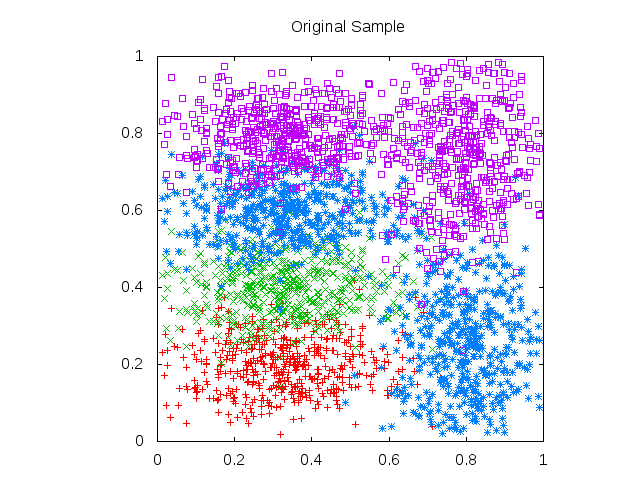
\includegraphics[scale=0.35]{big_samples.png}
	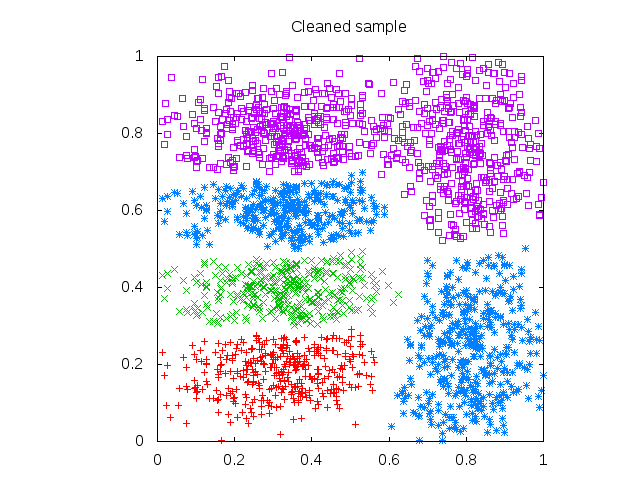
\includegraphics[scale=0.35]{cleaned_samples.png}
\end{center}

\paragraph{Seconde étape}
Puis on supprimer les exemples qui ne sont pas très révélateurs.
\begin{center}
	\begin{algorithm}[H]
		\KwIn{$S$}
		\KwOut{STORAGE}
		STORAGE $\gets \emptyset$\; 
		Choisir aléatoirement un exemple de $S$ et le mettre dans STORAGE\;
		\Repeat{stabilisation de STORAGE}{
			\For{$x \in S$} {
				\If{$x$ n'est pas correctement classé en utilisant 1-NN avec STORAGE}{
					STORAGE $\gets$ STORAGE $\cup \; \{x\}$
				}
			}
		}
		\KwResult{STORAGE}
		\caption{Plus proche voisin condensé (CNN)}
	\end{algorithm}
	
	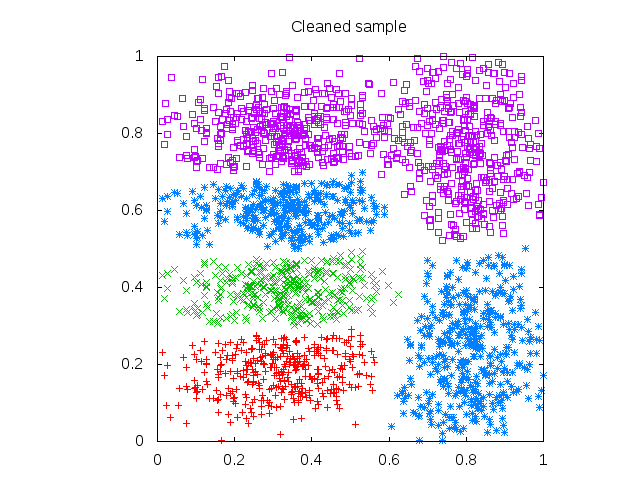
\includegraphics[scale=0.35]{cleaned_samples.png}
	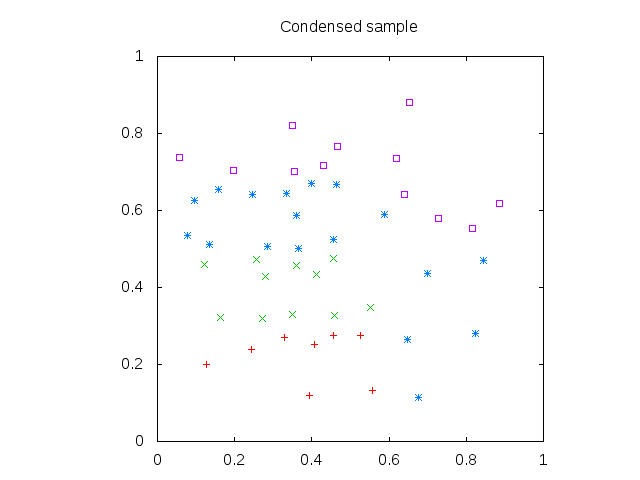
\includegraphics[scale=0.35]{condensed_samples.png}
\end{center}

\paragraph{Augmenter la rapidité}
En 2D ou en 3D on peut utiliser des diagrammes de Voronoi ou encore des graphes de proximité.
En plus grande dimension on peut utiliser les structures de données suivantes : ball-trees, kd-trees, metric-trees, quadtrees et R-trees.
	\chapter{Analyse en composantes principales}

\myminitoc

\sect{Introduction - Maximisation de la variance}

L'\textbf{analyse de composante principale (PCA)} est une réduction de la dimension. Elle projette un ensemble de points vivant dans un espace de dimension {\boldmath $d$} sur un sous-espace de dimension {\boldmath $M$}~$< d$. Si $M = 2$ alors on peut visualiser les données. L'analyse génère de nouvelles features qui sont décorrélés et qui un sens qui permet de bien discriminer les données.

\begin{center}
	\begin{tikzpicture}[thick]
		\draw[purple, very thick] (0, -0.846) -- (8, 3.804);
		\draw[greenTikz] (0.491, 0.039) -- (0.751, -0.409);
		\draw[fill=red] (0.491, 0.039) circle (0.15);
		\draw[fill=greenTikz] (0.751, -0.409) circle (0.15);
		\draw[greenTikz] (3.370, 0.587) -- (3.141, 0.980);
		\draw[fill=red] (3.370, 0.587) circle (0.15);
		\draw[fill=greenTikz] (3.141, 0.980) circle (0.15);
		\draw[greenTikz] (1.769, -0.248) -- (1.582, 0.073);
		\draw[fill=red] (1.769, -0.248) circle (0.15);
		\draw[fill=greenTikz] (1.582, 0.073) circle (0.15);
		\draw[greenTikz] (5.370, 3.037) -- (5.701, 2.468);
		\draw[fill=red] (5.370, 3.037) circle (0.15);
		\draw[fill=greenTikz] (5.701, 2.468) circle (0.15);
		\draw[greenTikz] (6.241, 2.376) -- (6.064, 2.679);
		\draw[fill=red] (6.241, 2.376) circle (0.15);
		\draw[fill=greenTikz] (6.064, 2.679) circle (0.15);
	\end{tikzpicture} \\
	Ici $d=2$ et $M=1$.
	\vspace{1mm}
\end{center}

Supposons que notre ensemble d'entraînement a une moyenne nulle, (cela peut être obtenu en remplaçant les $x_i$ par $x_i - \bar{x}$). PCA cherche une transformation linéaire $U$ qui à $x_i$ associera le nouveau point :
$$ t_i = U^\trans x_i $$
Où $U = (u_1, ..., u_M)$ est une matrice de dimension $d \times M$. Les vecteurs $u_j$ représentent une base de notre sous espace de $R^d$. De plus on souhaite que la base soit orthonormale. On obtient donc la contrainte suivante :
$$ U^\trans U = I_M $$
On peut aussi définir la reconstruction d'un point du nouveau sous-espace par $\hat{x}_i = U t_i$. Dans ce cas on veut minimiser l'erreur quadratique moyenne $J(U)$ entre $x$ et $\hat{x}$ tout en essayant de garder $M$ aussi petit que possible.
$$ \begin{array}{lll}
\displaystyle \min_U J(U)
& = & \displaystyle \min_U~\dfrac{1}{n} \sum_i (x_i - \hat{x}_i)² \\
& = & \displaystyle \min_U~\dfrac{1}{n} \sum_i (x_i - UU^\trans x_i)^\trans (x_i - UU^\trans x_i) \\
& = & \displaystyle \min_U~\dfrac{1}{n} \sum_i (x_i^\trans x_i - 2 xi^\trans UU^\trans x_i + x_i^\trans U U^\trans U U^\trans x_i)
\end{array} $$
On utilise alors la contrainte $U^\trans U = I_M$ :
$$ \begin{array}{lll}
\displaystyle \min_U J(U)
& = & \displaystyle \min_U~\dfrac{1}{n} \sum_i (x_i^\trans x_i - xi^\trans UU^\trans x_i) \\
& = & \displaystyle \min_U~\dfrac{1}{n} \sum_i (x_i^\trans x_i - t_i^\trans t_i) \\
& = & \displaystyle \min_U~tr \left( \dfrac{1}{n} \sum_i x_i x_i^\trans - t_i t_i^\trans \right) \\
& = & \displaystyle \min_U~tr \left( \dfrac{1}{n} \sum_i x_i x_i^\trans - U^\trans x_i x_i^\trans U \right) \\
& = & \displaystyle \min_U~tr \left( \dfrac{1}{n} \sum_i x_i x_i^\trans \right) - tr \left( \dfrac{1}{n} \sum_i U^\trans x_i x_i^\trans U \right) \\
& = & \displaystyle \min_U~tr \left( \dfrac{1}{n} \sum_i x_i x_i^\trans \right) - tr \left( U^\trans \left( \dfrac{1}{n} \sum_i x_i x_i^\trans \right) U \right) \\
& = & \displaystyle \min_U~tr \left( \Sigma \right) - tr \left( U^\trans \Sigma U \right)
\end{array} $$
Où {\boldmath $\Sigma$} est la \textbf{matrice de covariance} des données d'origine et $U^\trans \Sigma U$ est la matrice de covariance dans le nouvelle espace. \\
Comme $tr(\Sigma)$ ne dépend pas de $U$ minimiser $J(U)$ revient à maximiser $tr(U^\trans \Sigma U)$. On obtient donc le problème suivant :
\begin{center}
	\fbox{
	\parbox{7cm}{
	$$ \max_{u_1, ..., u_M} \sum_j u_j^\trans \Sigma u_j $$
	\vspace{-4mm}
	$$ \text{s.t.} \quad \forall j, k \in \{ 1, ..., M \}, \, u_j^\trans u_k = \delta_{j, k} $$
	\vspace{-4mm}
	}
	}
\end{center}

\sect{Solution de forme fermée}

La matrice de covariance $\Sigma$ est symétrique donc en utilisant le théorème spectrale on obtient l'existence d'une matrice diagonale $D = diag(\lambda_1, ..., \lambda_d)$ et l'existence d'une matrice orthogonale $V$ tel que $\Sigma = V D V^\trans$. On ordonne les valeurs propres de $\Sigma$ de telle sorte que $\lambda_1 \geqslant ... \geqslant \lambda_d$. \\
On cherche donc à maximiser la valeur suivante :
$$ \begin{array}{lll}
\displaystyle \sum_j u_j^\trans \Sigma u_j
& = & \displaystyle \sum_j u_j^\trans V D V^\trans u_j \\
& = & \displaystyle \sum_j \left( V^\trans u_j \right)^\trans D \left( V^\trans u_j \right) \\
& = & \displaystyle \sum_{i, j} \left( v_i^\trans u_j \right) \lambda_i \left( v_i^\trans u_j \right) \\
& = & \displaystyle \sum_{i, j} \lambda_i \left( v_i^\trans u_j \right)^2 \\
\end{array} $$
Comme les $(u_j)$ forment une famille orthonormale, on peut la compléter par des vecteurs $w_{M+1}, ..., w_d$ pour former une base orthonormale. Ainsi la matrice formé des colonnes $W = (u_1, ..., u_M, w_{M+1}, ..., w_d)$ est une matrice orthogonale. Comme $V$ est aussi orthogonale, le produit $V^\trans W$ est une matrice orthogonale. Puis, en utilisant le fait que les lignes d'une matrice orthogonale sont de norme 1, on obtient :
$$ \forall i, \quad \alpha_i = \sum_{j = 1}^M \left( v_i^\trans u_j \right)^2 = 1 - \sum_{j = M+1}^d \left( v_i^\trans w_j \right)^2 \leqslant 1 $$
De plus, les vecteurs $(v_i)$ formant une base orthonormé, on obtient $\sum_i \left( v_i^\trans u_j \right)^2 = u_j^\trans u_j = 1$. D'où :
$$ \sum_i \alpha_i = \sum_{i, j} \left( v_i^\trans u_j \right)^2 = M $$
Notre problème s'écrit alors :
$$ \max_\alpha \sum_i \lambda_i \alpha_i $$
\vspace{-2mm}
$$ \text{s.t.} \quad \left\{ \begin{array}{l}
\forall i, \, \alpha_i \leqslant 1 \\
\sum_i \alpha_i = M
\end{array} \right. $$
Une solution optimale est alors $\alpha_i = 1$ si $i \leqslant M$ et $\alpha_i = 0$ si $i > M$. Ces valeurs de $\alpha_i$ peuvent être obtenue avec $u_j = v_j$. \\
{\boldmath \textbf{Trouver} $U$ \textbf{revient alors à trouver les vecteurs propres correspondant aux plus grandes valeurs propres de} $\Sigma$}.

\paragraph{Qualité de la projection}
Pour ne pas perdre d'information on peut prendre $M$ le nombre de valeurs propres non nulles de $\Sigma$. La somme des valeurs propres correspond à la variance de données. Si on s'autorise une perte de variance, on peut alors définir le ratio de la variance conservée :
$$ \dfrac{\lambda_1 + ... + \lambda_M}{\lambda_1 + ... + \lambda_d} $$
Plus ce ratio est élevé meilleur est notre projection.

\paragraph{Complexité}
La complexité de PCA est alors la complexité de la décomposition en vecteur propre d'une matrice de taille $d \times d$. La complexité est donc en $\mathcal{O}(d^3)$. \\
Cependant si $M$ est suffisamment petit on peut utiliser la méthode de la puissance pour une complexité en $\mathcal{O}(Md^2)$.

\paragraph{Limitations}
Une première limitation est que PCA est très sensibles aux valeurs aberrantes.
\begin{center}
	\begin{tikzpicture}[thick, >={latex}]
		\draw[greenTikz, very thick] (0, 0.479) -- (7.155, 2.809);
		\draw[->] (6.3, 1.8) node[below] {\footnotesize composante principale apprise} -- (6, 2.35);
		\draw[blue, very thick] (0, 0) -- (7.155, 3.578);
		\draw[fill=red] (2.712, 1.356) circle (0.15);
		\draw[fill=red] (6.431, 3.215) circle (0.15);
		\draw[fill=red] (5.061, 2.531) circle (0.15);
		\draw[fill=red] (0.330, 0.165) circle (0.15);
		\draw[fill=red] (6.326, 3.163) circle (0.15);
		\draw[fill=red] (1.298, 0.649) circle (0.15);
		\draw[fill=red] (0.059, 0.029) circle (0.15);
		\draw[fill=red] (0.852, 0.426) circle (0.15);
		\draw[fill=red] (6.557, 3.278) circle (0.15);
		\draw[fill=red] (5.409, 2.704) circle (0.15);
		\draw[fill=red] (2.209, 1.105) circle (0.15);
		\draw[fill=red] (2.868, 1.434) circle (0.15);
		\draw[fill=red] (2.291, 1.146) circle (0.15);
		\draw[fill=red] (5.678, 2.839) circle (0.15);
		\draw[fill=red] (3.428, 1.714) circle (0.15);
		\draw[fill=red] (4.888, 0.203) circle (0.15);
		\draw[fill=red] (6.743, 0.796) circle (0.15);
		\draw[fill=red] (0.013, 3.395) circle (0.15);
		\draw[fill=red] (3.097, 0.528) circle (0.15);
	\end{tikzpicture}
\end{center}
De plus PCA réalise une transformation linéaire et n'est pas capable de détecter des relations polynomiale entre les différentes features. PCA se contente de placer les points les plus différents loin des autres afin de conserver la variance dans un espace de faible dimension. Il serait bien que PCA essaye aussi de garder proche les points similaires. Cela nous amène au besoin d'une réduction de dimension non linéaire.

\paragraph{PCA avec noyau}
Pour obtenir une transformation non linéaire on peut utiliser un noyau $K$ tel que $K(x, x')$ est grand lorsque $x$ et $x'$ sont similaires. Si on possède $m$ exemples alors grâce à ce noyau on peut construire la matrice de Gram de taille $m \times m$ tel que $M_{ij} = K(x_i, x_j)$. On utilise alors PCA sur cette nouvelle matrice ce qui nous donnera une transformation non linéaire.
\begin{center}
	\begin{tikzpicture}[scale=0.3]
		\draw[gray!40] (-9.000, -9.000) -- (9.000, -9.000);
\draw[gray!40] (-9.000, -9.000) -- (-9.000, 9.000);
\draw[gray!40] (-9.000, -6.750) -- (9.000, -6.750);
\draw[gray!40] (-6.750, -9.000) -- (-6.750, 9.000);
\draw[gray!40] (-9.000, -4.500) -- (9.000, -4.500);
\draw[gray!40] (-4.500, -9.000) -- (-4.500, 9.000);
\draw[gray!40] (-9.000, -2.250) -- (9.000, -2.250);
\draw[gray!40] (-2.250, -9.000) -- (-2.250, 9.000);
\draw[gray!40] (-9.000, 0.000) -- (9.000, 0.000);
\draw[gray!40] (0.000, -9.000) -- (0.000, 9.000);
\draw[gray!40] (-9.000, 2.250) -- (9.000, 2.250);
\draw[gray!40] (2.250, -9.000) -- (2.250, 9.000);
\draw[gray!40] (-9.000, 4.500) -- (9.000, 4.500);
\draw[gray!40] (4.500, -9.000) -- (4.500, 9.000);
\draw[gray!40] (-9.000, 6.750) -- (9.000, 6.750);
\draw[gray!40] (6.750, -9.000) -- (6.750, 9.000);
\draw[gray!40] (-9.000, 9.000) -- (9.000, 9.000);
\draw[gray!40] (9.000, -9.000) -- (9.000, 9.000);
\node[red] at (9.610, -0.184) {$\bullet$};
\node[red] at (-3.986, -8.917) {$\bullet$};
\node[red] at (-1.438, -9.539) {$\bullet$};
\node[red] at (-2.630, 8.676) {$\bullet$};
\node[red] at (8.649, 4.146) {$\bullet$};
\node[red] at (-0.652, 9.831) {$\bullet$};
\node[red] at (4.581, 8.331) {$\bullet$};
\node[red] at (-5.639, 8.039) {$\bullet$};
\node[red] at (9.098, -3.705) {$\bullet$};
\node[red] at (6.531, -6.630) {$\bullet$};
\node[red] at (0.732, 9.733) {$\bullet$};
\node[red] at (-2.497, 9.188) {$\bullet$};
\node[red] at (-9.689, -1.214) {$\bullet$};
\node[red] at (7.267, -5.607) {$\bullet$};
\node[red] at (0.203, 9.303) {$\bullet$};
\node[red] at (-1.376, 9.484) {$\bullet$};
\node[red] at (9.816, -1.747) {$\bullet$};
\node[red] at (-3.118, -9.341) {$\bullet$};
\node[red] at (-2.433, 8.935) {$\bullet$};
\node[red] at (9.042, -1.100) {$\bullet$};
\node[red] at (-7.350, 5.381) {$\bullet$};
\node[red] at (5.325, 7.763) {$\bullet$};
\node[red] at (2.333, -8.779) {$\bullet$};
\node[red] at (-5.960, 7.986) {$\bullet$};
\node[red] at (9.268, 0.311) {$\bullet$};
\node[red] at (-3.808, -8.178) {$\bullet$};
\node[red] at (-7.775, 5.113) {$\bullet$};
\node[red] at (-3.092, -9.475) {$\bullet$};
\node[red] at (-5.538, -7.574) {$\bullet$};
\node[red] at (-1.031, 9.546) {$\bullet$};
\node[red] at (5.427, 7.259) {$\bullet$};
\node[red] at (8.257, 5.319) {$\bullet$};
\node[red] at (-9.411, -1.824) {$\bullet$};
\node[red] at (2.413, -8.795) {$\bullet$};
\node[red] at (9.378, 1.910) {$\bullet$};
\node[red] at (8.327, -4.382) {$\bullet$};
\node[red] at (-4.915, -8.438) {$\bullet$};
\node[red] at (3.635, -8.700) {$\bullet$};
\node[red] at (-6.059, 6.752) {$\bullet$};
\node[red] at (-2.112, 8.845) {$\bullet$};
\node[red] at (6.612, 6.468) {$\bullet$};
\node[red] at (-6.923, 7.090) {$\bullet$};
\node[red] at (1.950, 8.969) {$\bullet$};
\node[red] at (-3.773, -8.185) {$\bullet$};
\node[red] at (9.400, 0.624) {$\bullet$};
\node[red] at (8.058, 4.049) {$\bullet$};
\node[red] at (7.143, 5.499) {$\bullet$};
\node[red] at (2.864, 8.660) {$\bullet$};
\node[red] at (3.348, 9.000) {$\bullet$};
\node[red] at (-8.862, -1.781) {$\bullet$};
\node[red] at (2.301, 9.185) {$\bullet$};
\node[red] at (9.221, -0.052) {$\bullet$};
\node[red] at (-8.659, -2.847) {$\bullet$};
\node[red] at (-3.573, 9.193) {$\bullet$};
\node[red] at (8.881, -2.580) {$\bullet$};
\node[red] at (0.386, 9.219) {$\bullet$};
\node[red] at (-7.276, 6.472) {$\bullet$};
\node[red] at (5.721, -8.071) {$\bullet$};
\node[red] at (6.843, -5.962) {$\bullet$};
\node[red] at (4.241, -8.820) {$\bullet$};
\node[red] at (-7.964, -5.719) {$\bullet$};
\node[red] at (7.142, 6.481) {$\bullet$};
\node[red] at (7.901, -5.730) {$\bullet$};
\node[red] at (9.485, -2.513) {$\bullet$};
\node[red] at (-9.355, 1.257) {$\bullet$};
\node[red] at (2.600, -9.318) {$\bullet$};
\node[red] at (8.548, 4.185) {$\bullet$};
\node[red] at (-2.466, -9.046) {$\bullet$};
\node[red] at (8.073, -4.414) {$\bullet$};
\node[red] at (-8.599, -4.563) {$\bullet$};
\node[red] at (-7.709, 4.910) {$\bullet$};
\node[red] at (-9.131, -1.883) {$\bullet$};
\node[red] at (9.569, -1.495) {$\bullet$};
\node[red] at (9.032, 1.457) {$\bullet$};
\node[red] at (-7.541, -5.504) {$\bullet$};
\node[red] at (7.107, 6.899) {$\bullet$};
\node[red] at (6.716, -6.301) {$\bullet$};
\node[red] at (-8.901, 3.407) {$\bullet$};
\node[red] at (9.985, -0.023) {$\bullet$};
\node[red] at (-5.764, -7.761) {$\bullet$};
\node[red] at (9.288, -2.593) {$\bullet$};
\node[red] at (4.497, -8.162) {$\bullet$};
\node[red] at (7.584, -6.027) {$\bullet$};
\node[red] at (-2.505, 8.983) {$\bullet$};
\node[red] at (-9.895, 0.587) {$\bullet$};
\node[red] at (5.825, 7.427) {$\bullet$};
\node[red] at (-6.985, 6.197) {$\bullet$};
\node[red] at (-9.130, 2.036) {$\bullet$};
\node[red] at (-2.845, -8.700) {$\bullet$};
\node[red] at (4.152, 8.814) {$\bullet$};
\node[blue] at (-1.305, -3.207) {$\bullet$};
\node[blue] at (1.183, 3.779) {$\bullet$};
\node[blue] at (-2.702, -2.197) {$\bullet$};
\node[blue] at (1.143, 2.942) {$\bullet$};
\node[blue] at (-0.437, -3.024) {$\bullet$};
\node[blue] at (-3.511, -0.416) {$\bullet$};
\node[blue] at (2.291, -2.656) {$\bullet$};
\node[blue] at (3.857, -0.416) {$\bullet$};
\node[blue] at (2.825, -1.752) {$\bullet$};
\node[blue] at (2.262, 2.072) {$\bullet$};
\node[blue] at (-3.596, 0.269) {$\bullet$};
\node[blue] at (3.641, 1.626) {$\bullet$};
\node[blue] at (3.370, -1.722) {$\bullet$};
\node[blue] at (3.165, -0.770) {$\bullet$};
\node[blue] at (1.324, 3.227) {$\bullet$};
\node[blue] at (3.785, 0.977) {$\bullet$};
\node[blue] at (0.562, 3.806) {$\bullet$};
\node[blue] at (-3.706, 1.321) {$\bullet$};
\node[blue] at (3.474, 0.369) {$\bullet$};
\node[blue] at (-3.088, -1.221) {$\bullet$};
\node[blue] at (3.670, 0.091) {$\bullet$};
\node[blue] at (3.844, 0.776) {$\bullet$};
\node[blue] at (1.608, -2.943) {$\bullet$};
\node[blue] at (-3.005, 0.169) {$\bullet$};
\node[blue] at (-3.073, 1.575) {$\bullet$};
\node[blue] at (-1.598, -2.952) {$\bullet$};
\node[blue] at (-0.957, 3.772) {$\bullet$};
\node[blue] at (-3.295, 2.012) {$\bullet$};
\node[blue] at (-3.025, 2.052) {$\bullet$};
\node[blue] at (0.113, 3.327) {$\bullet$};
\node[greenTikz] at (0.441, -0.728) {$\bullet$};
\node[greenTikz] at (-0.372, 0.872) {$\bullet$};
\node[greenTikz] at (-0.000, -0.000) {$\bullet$};
\node[greenTikz] at (0.624, 0.174) {$\bullet$};
\node[greenTikz] at (-0.552, -0.595) {$\bullet$};
\node[greenTikz] at (-0.581, 0.385) {$\bullet$};
\node[greenTikz] at (-0.018, -0.470) {$\bullet$};
\node[greenTikz] at (0.519, -0.755) {$\bullet$};

	\end{tikzpicture}
	\begin{tikzpicture}[scale=1.4]
		\draw[gray!40] (-0.150,  -0) -- (-0.170, -0.086) -- (-0.196, -0.103) -- (-0.227, -0.125) -- (-0.263, -0.150) -- (-0.302, -0.176) -- (-0.339, -0.202) -- (-0.370, -0.223) -- (-0.390, -0.237) -- (-0.396, -0.240) -- (-0.388, -0.233) -- (-0.367, -0.216) -- (-0.337, -0.190) -- (-0.306, -0.160) -- (-0.278, -0.127) -- (-0.260, -0.094) -- (-0.252, -0.062) -- (-0.256, -0.032) -- (-0.270, -0.002) -- (-0.291, 0.029) -- (-0.314, 0.063) -- (-0.338, 0.100) -- (-0.359, 0.139) -- (-0.376, 0.179) -- (-0.387, 0.215) -- (-0.390, 0.243) -- (-0.384, 0.259) -- (-0.368, 0.260) -- (-0.343, 0.245) -- (-0.310, 0.215) -- (-0.274, 0.176);
\draw[gray!40] (-0.150,  -0) -- (-0.159, -0.078) -- (-0.168, -0.084) -- (-0.176, -0.089) -- (-0.183, -0.094) -- (-0.190, -0.099) -- (-0.196, -0.103) -- (-0.202, -0.109) -- (-0.208, -0.114) -- (-0.212, -0.120) -- (-0.215, -0.125) -- (-0.216, -0.130) -- (-0.214, -0.133) -- (-0.210, -0.136) -- (-0.205, -0.138) -- (-0.200, -0.142) -- (-0.197, -0.147) -- (-0.197, -0.156) -- (-0.202, -0.170) -- (-0.212, -0.190) -- (-0.226, -0.215) -- (-0.243, -0.245) -- (-0.261, -0.276) -- (-0.276, -0.304) -- (-0.287, -0.326) -- (-0.291, -0.337) -- (-0.286, -0.336) -- (-0.274, -0.321) -- (-0.255, -0.294) -- (-0.232, -0.259) -- (-0.207, -0.219);
\draw[gray!40] (-0.181,  -0) -- (-0.200, -0.105) -- (-0.219, -0.119) -- (-0.238, -0.134) -- (-0.257, -0.150) -- (-0.272, -0.164) -- (-0.281, -0.177) -- (-0.282, -0.185) -- (-0.273, -0.187) -- (-0.252, -0.182) -- (-0.221, -0.171) -- (-0.184, -0.153) -- (-0.146, -0.130) -- (-0.111, -0.105) -- (-0.085, -0.079) -- (-0.071, -0.053) -- (-0.071, -0.027) -- (-0.087, 0.001) -- (-0.116, 0.033) -- (-0.160, 0.075) -- (-0.216, 0.130) -- (-0.284, 0.201) -- (-0.361, 0.290) -- (-0.445, 0.393) -- (-0.527, 0.505) -- (-0.601, 0.612) -- (-0.657, 0.701) -- (-0.687, 0.757) -- (-0.686, 0.772) -- (-0.654, 0.742) -- (-0.596, 0.671);
\draw[gray!40] (-0.254,  -0) -- (-0.265, -0.151) -- (-0.268, -0.154) -- (-0.262, -0.151) -- (-0.248, -0.144) -- (-0.228, -0.135) -- (-0.204, -0.125) -- (-0.176, -0.115) -- (-0.146, -0.108) -- (-0.114, -0.103) -- (-0.079, -0.099) -- (-0.043, -0.097) -- (-0.007, -0.095) -- (0.026, -0.096) -- (0.052, -0.098) -- (0.067, -0.103) -- (0.068, -0.112) -- (0.052, -0.128) -- (0.020, -0.153) -- (-0.027, -0.187) -- (-0.086, -0.234) -- (-0.152, -0.291) -- (-0.219, -0.357) -- (-0.283, -0.428) -- (-0.339, -0.498) -- (-0.382, -0.559) -- (-0.409, -0.604) -- (-0.420, -0.628) -- (-0.414, -0.625) -- (-0.393, -0.596) -- (-0.360, -0.543);
\draw[gray!40] (-0.205,  -0) -- (-0.206, -0.116) -- (-0.199, -0.116) -- (-0.182, -0.114) -- (-0.154, -0.110) -- (-0.113, -0.104) -- (-0.060, -0.097) -- (0.006, -0.088) -- (0.085, -0.078) -- (0.172, -0.065) -- (0.264, -0.050) -- (0.355, -0.033) -- (0.437, -0.015) -- (0.505, 0.005) -- (0.553, 0.025) -- (0.576, 0.044) -- (0.574, 0.064) -- (0.547, 0.085) -- (0.493, 0.109) -- (0.413, 0.141) -- (0.308, 0.188) -- (0.176, 0.255) -- (0.021, 0.351) -- (-0.154, 0.480) -- (-0.341, 0.642) -- (-0.528, 0.828) -- (-0.702, 1.020) -- (-0.847, 1.196) -- (-0.949, 1.327) -- (-0.996, 1.391) -- (-0.985, 1.374);
\draw[gray!40] (-0.381,  -0) -- (-0.382, -0.234) -- (-0.362, -0.225) -- (-0.321, -0.206) -- (-0.262, -0.180) -- (-0.189, -0.150) -- (-0.103, -0.121) -- (-0.007, -0.095) -- (0.098, -0.073) -- (0.212, -0.057) -- (0.332, -0.044) -- (0.454, -0.036) -- (0.569, -0.031) -- (0.668, -0.030) -- (0.740, -0.032) -- (0.775, -0.038) -- (0.769, -0.049) -- (0.719, -0.064) -- (0.630, -0.085) -- (0.511, -0.115) -- (0.373, -0.156) -- (0.226, -0.214) -- (0.079, -0.292) -- (-0.063, -0.393) -- (-0.194, -0.520) -- (-0.314, -0.667) -- (-0.419, -0.823) -- (-0.506, -0.971) -- (-0.568, -1.090) -- (-0.600, -1.159) -- (-0.600, -1.163);
\draw[gray!40] (-0.215,  -0) -- (-0.195, -0.128) -- (-0.156, -0.119) -- (-0.095, -0.107) -- (-0.010, -0.092) -- (0.100, -0.077) -- (0.235, -0.061) -- (0.395, -0.044) -- (0.576, -0.025) -- (0.772, -0.004) -- (0.975, 0.021) -- (1.176, 0.050) -- (1.361, 0.082) -- (1.518, 0.116) -- (1.635, 0.151) -- (1.701, 0.184) -- (1.713, 0.215) -- (1.670, 0.242) -- (1.575, 0.265) -- (1.433, 0.287) -- (1.248, 0.311) -- (1.025, 0.347) -- (0.766, 0.407) -- (0.477, 0.506) -- (0.168, 0.655) -- (-0.151, 0.861) -- (-0.464, 1.115) -- (-0.752, 1.391) -- (-0.992, 1.651) -- (-1.164, 1.848) -- (-1.252, 1.942);
\draw[gray!40] (-0.360,  -0) -- (-0.346, -0.207) -- (-0.306, -0.193) -- (-0.241, -0.169) -- (-0.149, -0.140) -- (-0.032, -0.107) -- (0.111, -0.074) -- (0.281, -0.043) -- (0.478, -0.015) -- (0.697, 0.011) -- (0.932, 0.034) -- (1.167, 0.054) -- (1.385, 0.068) -- (1.563, 0.076) -- (1.680, 0.077) -- (1.722, 0.069) -- (1.684, 0.053) -- (1.570, 0.030) -- (1.397, 0.001) -- (1.183, -0.035) -- (0.948, -0.081) -- (0.708, -0.144) -- (0.472, -0.233) -- (0.246, -0.360) -- (0.028, -0.536) -- (-0.180, -0.761) -- (-0.376, -1.026) -- (-0.553, -1.305) -- (-0.700, -1.561) -- (-0.803, -1.751) -- (-0.853, -1.837);
\draw[gray!40] (-0.200,  -0) -- (-0.166, -0.137) -- (-0.108, -0.128) -- (-0.020, -0.114) -- (0.101, -0.099) -- (0.255, -0.082) -- (0.442, -0.066) -- (0.658, -0.048) -- (0.897, -0.028) -- (1.150, -0.004) -- (1.408, 0.025) -- (1.661, 0.060) -- (1.896, 0.099) -- (2.098, 0.142) -- (2.250, 0.185) -- (2.340, 0.228) -- (2.359, 0.266) -- (2.308, 0.300) -- (2.192, 0.328) -- (2.018, 0.349) -- (1.795, 0.366) -- (1.527, 0.385) -- (1.220, 0.417) -- (0.882, 0.478) -- (0.521, 0.584) -- (0.152, 0.747) -- (-0.209, 0.965) -- (-0.543, 1.221) -- (-0.828, 1.478) -- (-1.042, 1.691) -- (-1.168, 1.815);
\draw[gray!40] (-0.260,  -0) -- (-0.242, -0.089) -- (-0.202, -0.080) -- (-0.138, -0.066) -- (-0.044, -0.049) -- (0.082, -0.027) -- (0.248, -0.002) -- (0.456, 0.028) -- (0.707, 0.062) -- (0.996, 0.099) -- (1.309, 0.138) -- (1.625, 0.176) -- (1.915, 0.207) -- (2.148, 0.229) -- (2.295, 0.236) -- (2.340, 0.228) -- (2.280, 0.203) -- (2.128, 0.166) -- (1.906, 0.118) -- (1.640, 0.063) -- (1.353, -0.000) -- (1.063, -0.074) -- (0.778, -0.169) -- (0.502, -0.295) -- (0.237, -0.465) -- (-0.017, -0.684) -- (-0.254, -0.944) -- (-0.467, -1.224) -- (-0.645, -1.488) -- (-0.774, -1.693) -- (-0.844, -1.801);
\draw[gray!40] (-0.209,  -0) -- (-0.190, -0.193) -- (-0.149, -0.194) -- (-0.083, -0.187) -- (0.012, -0.174) -- (0.136, -0.157) -- (0.284, -0.137) -- (0.453, -0.117) -- (0.635, -0.096) -- (0.823, -0.076) -- (1.012, -0.054) -- (1.195, -0.031) -- (1.366, -0.006) -- (1.516, 0.020) -- (1.634, 0.049) -- (1.709, 0.077) -- (1.732, 0.105) -- (1.698, 0.130) -- (1.609, 0.152) -- (1.471, 0.169) -- (1.292, 0.183) -- (1.078, 0.194) -- (0.838, 0.211) -- (0.580, 0.241) -- (0.314, 0.296) -- (0.049, 0.382) -- (-0.200, 0.500) -- (-0.422, 0.640) -- (-0.603, 0.782) -- (-0.730, 0.900) -- (-0.797, 0.970);
\draw[gray!40] (-0.285,   0) -- (-0.280, 0.034) -- (-0.254, 0.045) -- (-0.203, 0.056) -- (-0.125, 0.066) -- (-0.014, 0.079) -- (0.135, 0.096) -- (0.325, 0.118) -- (0.556, 0.148) -- (0.822, 0.185) -- (1.112, 0.228) -- (1.403, 0.271) -- (1.669, 0.310) -- (1.884, 0.338) -- (2.021, 0.351) -- (2.067, 0.345) -- (2.018, 0.318) -- (1.886, 0.274) -- (1.688, 0.216) -- (1.447, 0.148) -- (1.184, 0.072) -- (0.914, -0.012) -- (0.649, -0.109) -- (0.394, -0.226) -- (0.154, -0.369) -- (-0.067, -0.540) -- (-0.267, -0.732) -- (-0.436, -0.929) -- (-0.569, -1.104) -- (-0.657, -1.231) -- (-0.695, -1.286);
\draw[gray!40] (-0.269,  -0) -- (-0.286, -0.334) -- (-0.290, -0.368) -- (-0.276, -0.388) -- (-0.241, -0.392) -- (-0.188, -0.384) -- (-0.118, -0.368) -- (-0.037, -0.349) -- (0.052, -0.331) -- (0.144, -0.317) -- (0.239, -0.305) -- (0.334, -0.294) -- (0.428, -0.282) -- (0.515, -0.266) -- (0.588, -0.248) -- (0.639, -0.227) -- (0.658, -0.206) -- (0.640, -0.188) -- (0.584, -0.173) -- (0.495, -0.162) -- (0.378, -0.156) -- (0.243, -0.152) -- (0.099, -0.146) -- (-0.047, -0.133) -- (-0.187, -0.108) -- (-0.313, -0.068) -- (-0.419, -0.014) -- (-0.498, 0.051) -- (-0.547, 0.116) -- (-0.562, 0.174) -- (-0.547, 0.212);
\draw[gray!40] (-0.369,   0) -- (-0.401, 0.211) -- (-0.420, 0.263) -- (-0.419, 0.310) -- (-0.394, 0.349) -- (-0.340, 0.377) -- (-0.254, 0.396) -- (-0.136, 0.407) -- (0.014, 0.415) -- (0.190, 0.423) -- (0.382, 0.434) -- (0.578, 0.447) -- (0.759, 0.460) -- (0.909, 0.467) -- (1.011, 0.462) -- (1.055, 0.443) -- (1.036, 0.405) -- (0.957, 0.351) -- (0.830, 0.282) -- (0.668, 0.203) -- (0.486, 0.115) -- (0.298, 0.019) -- (0.114, -0.085) -- (-0.059, -0.199) -- (-0.215, -0.322) -- (-0.351, -0.450) -- (-0.461, -0.577) -- (-0.541, -0.688) -- (-0.588, -0.769) -- (-0.600, -0.809) -- (-0.579, -0.800);
\draw[gray!40] (-0.284,  -0) -- (-0.327, -0.411) -- (-0.365, -0.489) -- (-0.396, -0.562) -- (-0.418, -0.629) -- (-0.431, -0.692) -- (-0.438, -0.756) -- (-0.442, -0.825) -- (-0.444, -0.899) -- (-0.444, -0.973) -- (-0.439, -1.040) -- (-0.427, -1.088) -- (-0.405, -1.109) -- (-0.375, -1.101) -- (-0.341, -1.067) -- (-0.310, -1.013) -- (-0.289, -0.950) -- (-0.282, -0.884) -- (-0.293, -0.823) -- (-0.320, -0.769) -- (-0.361, -0.720) -- (-0.409, -0.676) -- (-0.460, -0.630) -- (-0.506, -0.581) -- (-0.542, -0.523) -- (-0.563, -0.458) -- (-0.566, -0.385) -- (-0.550, -0.309) -- (-0.516, -0.235) -- (-0.467, -0.168) -- (-0.410, -0.114);
\draw[gray!40] (-0.381,   0) -- (-0.459, 0.370) -- (-0.540, 0.494) -- (-0.617, 0.623) -- (-0.682, 0.749) -- (-0.729, 0.863) -- (-0.752, 0.959) -- (-0.751, 1.036) -- (-0.727, 1.094) -- (-0.683, 1.137) -- (-0.625, 1.167) -- (-0.557, 1.182) -- (-0.485, 1.180) -- (-0.414, 1.156) -- (-0.349, 1.106) -- (-0.296, 1.027) -- (-0.259, 0.920) -- (-0.241, 0.791) -- (-0.244, 0.646) -- (-0.266, 0.496) -- (-0.306, 0.346) -- (-0.357, 0.202) -- (-0.413, 0.066) -- (-0.469, -0.060) -- (-0.516, -0.173) -- (-0.549, -0.272) -- (-0.563, -0.350) -- (-0.557, -0.404) -- (-0.530, -0.429) -- (-0.485, -0.426) -- (-0.429, -0.398);
\draw[gray!40] (-0.207,  -0) -- (-0.242, -0.286) -- (-0.281, -0.365) -- (-0.324, -0.460) -- (-0.373, -0.573) -- (-0.428, -0.710) -- (-0.491, -0.873) -- (-0.562, -1.062) -- (-0.639, -1.267) -- (-0.717, -1.474) -- (-0.788, -1.662) -- (-0.843, -1.809) -- (-0.876, -1.899) -- (-0.886, -1.924) -- (-0.874, -1.888) -- (-0.844, -1.801) -- (-0.806, -1.680) -- (-0.763, -1.540) -- (-0.723, -1.394) -- (-0.686, -1.250) -- (-0.654, -1.113) -- (-0.624, -0.983) -- (-0.595, -0.860) -- (-0.563, -0.741) -- (-0.527, -0.628) -- (-0.486, -0.521) -- (-0.441, -0.422) -- (-0.392, -0.332) -- (-0.341, -0.255) -- (-0.293, -0.191) -- (-0.248, -0.141);
\draw[gray!40] (-0.274,   0) -- (-0.343, 0.276) -- (-0.426, 0.401) -- (-0.520, 0.548) -- (-0.622, 0.714) -- (-0.728, 0.895) -- (-0.834, 1.084) -- (-0.936, 1.278) -- (-1.032, 1.468) -- (-1.119, 1.646) -- (-1.190, 1.801) -- (-1.243, 1.920) -- (-1.270, 1.990) -- (-1.267, 1.999) -- (-1.232, 1.940) -- (-1.168, 1.815) -- (-1.080, 1.632) -- (-0.978, 1.407) -- (-0.873, 1.159) -- (-0.774, 0.908) -- (-0.689, 0.672) -- (-0.621, 0.464) -- (-0.568, 0.288) -- (-0.527, 0.145) -- (-0.492, 0.035) -- (-0.457, -0.047) -- (-0.419, -0.103) -- (-0.378, -0.137) -- (-0.335, -0.152) -- (-0.290, -0.152) -- (-0.248, -0.141);
\node[greenTikz] at (2.292, 0.264) {$\bullet$};
\node[greenTikz] at (2.175, 0.164) {$\bullet$};
\node[greenTikz] at (2.340, 0.228) {$\bullet$};
\node[greenTikz] at (2.352, 0.262) {$\bullet$};
\node[greenTikz] at (2.217, 0.197) {$\bullet$};
\node[greenTikz] at (2.228, 0.174) {$\bullet$};
\node[greenTikz] at (2.312, 0.234) {$\bullet$};
\node[greenTikz] at (2.286, 0.269) {$\bullet$};
\node[blue] at (1.050, 0.067) {$\bullet$};
\node[blue] at (0.977, -0.063) {$\bullet$};
\node[blue] at (1.094, 0.036) {$\bullet$};
\node[blue] at (1.381, 0.049) {$\bullet$};
\node[blue] at (1.264, 0.117) {$\bullet$};
\node[blue] at (1.166, 0.005) {$\bullet$};
\node[blue] at (1.270, 0.254) {$\bullet$};
\node[blue] at (1.377, 0.407) {$\bullet$};
\node[blue] at (1.508, 0.332) {$\bullet$};
\node[blue] at (1.580, 0.186) {$\bullet$};
\node[blue] at (1.151, -0.009) {$\bullet$};
\node[blue] at (1.261, 0.268) {$\bullet$};
\node[blue] at (1.310, 0.357) {$\bullet$};
\node[blue] at (1.653, 0.377) {$\bullet$};
\node[blue] at (1.228, 0.019) {$\bullet$};
\node[blue] at (1.350, 0.335) {$\bullet$};
\node[blue] at (0.985, -0.085) {$\bullet$};
\node[blue] at (0.999, -0.040) {$\bullet$};
\node[blue] at (1.574, 0.365) {$\bullet$};
\node[blue] at (1.222, 0.029) {$\bullet$};
\node[blue] at (1.493, 0.385) {$\bullet$};
\node[blue] at (1.354, 0.353) {$\bullet$};
\node[blue] at (1.258, 0.207) {$\bullet$};
\node[blue] at (1.405, 0.022) {$\bullet$};
\node[blue] at (1.180, -0.025) {$\bullet$};
\node[blue] at (1.109, 0.066) {$\bullet$};
\node[blue] at (0.872, -0.130) {$\bullet$};
\node[blue] at (0.988, -0.053) {$\bullet$};
\node[blue] at (1.065, -0.045) {$\bullet$};
\node[blue] at (1.202, -0.035) {$\bullet$};
\node[red] at (-1.222, 1.865) {$\bullet$};
\node[red] at (-0.395, -0.240) {$\bullet$};
\node[red] at (-0.316, -0.168) {$\bullet$};
\node[red] at (-0.808, -1.732) {$\bullet$};
\node[red] at (-0.579, 0.282) {$\bullet$};
\node[red] at (-0.867, -1.840) {$\bullet$};
\node[red] at (-0.598, -0.792) {$\bullet$};
\node[red] at (-0.489, -0.839) {$\bullet$};
\node[red] at (-1.102, 1.610) {$\bullet$};
\node[red] at (-0.662, 0.714) {$\bullet$};
\node[red] at (-0.796, -1.620) {$\bullet$};
\node[red] at (-0.838, -1.790) {$\bullet$};
\node[red] at (-0.220, -0.134) {$\bullet$};
\node[red] at (-0.811, 1.018) {$\bullet$};
\node[red] at (-0.843, -1.773) {$\bullet$};
\node[red] at (-0.891, -1.916) {$\bullet$};
\node[red] at (-1.263, 1.937) {$\bullet$};
\node[red] at (-0.385, -0.230) {$\bullet$};
\node[red] at (-0.838, -1.799) {$\bullet$};
\node[red] at (-1.268, 1.998) {$\bullet$};
\node[red] at (-0.344, -0.468) {$\bullet$};
\node[red] at (-0.585, -0.645) {$\bullet$};
\node[red] at (-0.289, 0.031) {$\bullet$};
\node[red] at (-0.465, -0.769) {$\bullet$};
\node[red] at (-1.150, 1.745) {$\bullet$};
\node[red] at (-0.384, -0.239) {$\bullet$};
\node[red] at (-0.325, -0.420) {$\bullet$};
\node[red] at (-0.381, -0.227) {$\bullet$};
\node[red] at (-0.323, -0.195) {$\bullet$};
\node[red] at (-0.890, -1.909) {$\bullet$};
\node[red] at (-0.574, -0.587) {$\bullet$};
\node[red] at (-0.539, -0.007) {$\bullet$};
\node[red] at (-0.220, -0.133) {$\bullet$};
\node[red] at (-0.292, 0.035) {$\bullet$};
\node[red] at (-0.869, 1.124) {$\bullet$};
\node[red] at (-1.007, 1.418) {$\bullet$};
\node[red] at (-0.369, -0.224) {$\bullet$};
\node[red] at (-0.349, 0.118) {$\bullet$};
\node[red] at (-0.430, -0.686) {$\bullet$};
\node[red] at (-0.854, -1.848) {$\bullet$};
\node[red] at (-0.562, -0.351) {$\bullet$};
\node[red] at (-0.411, -0.603) {$\bullet$};
\node[red] at (-0.712, -1.357) {$\bullet$};
\node[red] at (-0.384, -0.239) {$\bullet$};
\node[red] at (-1.106, 1.641) {$\bullet$};
\node[red] at (-0.566, 0.256) {$\bullet$};
\node[red] at (-0.541, -0.150) {$\bullet$};
\node[red] at (-0.654, -1.132) {$\bullet$};
\node[red] at (-0.637, -1.037) {$\bullet$};
\node[red] at (-0.210, -0.133) {$\bullet$};
\node[red] at (-0.694, -1.274) {$\bullet$};
\node[red] at (-1.197, 1.846) {$\bullet$};
\node[red] at (-0.209, -0.126) {$\bullet$};
\node[red] at (-0.718, -1.476) {$\bullet$};
\node[red] at (-1.221, 1.882) {$\bullet$};
\node[red] at (-0.830, -1.736) {$\bullet$};
\node[red] at (-0.389, -0.545) {$\bullet$};
\node[red] at (-0.482, 0.368) {$\bullet$};
\node[red] at (-0.742, 0.885) {$\bullet$};
\node[red] at (-0.370, 0.155) {$\bullet$};
\node[red] at (-0.211, -0.116) {$\bullet$};
\node[red] at (-0.556, -0.289) {$\bullet$};
\node[red] at (-0.833, 1.045) {$\bullet$};
\node[red] at (-1.234, 1.879) {$\bullet$};
\node[red] at (-0.206, -0.154) {$\bullet$};
\node[red] at (-0.293, 0.032) {$\bullet$};
\node[red] at (-0.577, 0.264) {$\bullet$};
\node[red] at (-0.369, -0.218) {$\bullet$};
\node[red] at (-0.985, 1.386) {$\bullet$};
\node[red] at (-0.207, -0.114) {$\bullet$};
\node[red] at (-0.315, -0.408) {$\bullet$};
\node[red] at (-0.217, -0.133) {$\bullet$};
\node[red] at (-1.289, 1.994) {$\bullet$};
\node[red] at (-0.936, 1.304) {$\bullet$};
\node[red] at (-0.212, -0.120) {$\bullet$};
\node[red] at (-0.550, -0.334) {$\bullet$};
\node[red] at (-0.705, 0.803) {$\bullet$};
\node[red] at (-0.238, -0.240) {$\bullet$};
\node[red] at (-1.175, 1.765) {$\bullet$};
\node[red] at (-0.319, -0.191) {$\bullet$};
\node[red] at (-1.233, 1.882) {$\bullet$};
\node[red] at (-0.410, 0.232) {$\bullet$};
\node[red] at (-0.789, 0.955) {$\bullet$};
\node[red] at (-0.834, -1.787) {$\bullet$};
\node[red] at (-0.210, -0.139) {$\bullet$};
\node[red] at (-0.578, -0.549) {$\bullet$};
\node[red] at (-0.389, -0.557) {$\bullet$};
\node[red] at (-0.208, -0.175) {$\bullet$};
\node[red] at (-0.381, -0.231) {$\bullet$};
\node[red] at (-0.604, -0.875) {$\bullet$};

	\end{tikzpicture}
\end{center}
Ici on part de l'ensemble de points de l'image de gauche. La séparation est clairement non linéaire, PCA ne fonctionnera donc pas sur cet échantillon. On utilise alors un noyau gaussien défini par :
$$ K(x, y) = \exp \left( - \dfrac{\| x - y \|_2^2}{2 \sigma^2} \right) $$
En utilisant KPCA (PCA avec ce noyau) on projette nos points sur un nouvel espace de dimension 2 situé à droite. La transformation entre l'espace de gauche et l'espace de droite n'est clairement pas linéaire. La première composante de notre nouvel espace nous permet de bien distinguer les 3 cercles.

\paragraph{t-SNE}
L'algorithme t-SNE pour t-distributed stochastic neighbor embedding construit une distributions de probabilité $P$ sur toute les paires d'exemples de notre ensemble de données tel que la probabilité d'une paire de points est grande lorsque ces points sont proches et la probabilité d'une paire de points est faible lorsque les points sont éloignés. Cette distribution est typiquement obtenue avec un noyau. \\
Puis l'algorithme construit une transformation qui à chaque point de notre ensemble de départ associe un nouveau point dans un nouvel espace de plus faible dimension $M \ll d$. On obtient de la même manière des distributions de probabilité $Q_i$ sur ce nouvel espace. Le but de t-SNE est alors de minimiser la divergence KL entre $P$ et $Q$ (en utilisant une descente de gradient). \\
Pour la distribution un exemple classique est le suivant :
$$ p_{ij} = \dfrac{p_{i|j} + p_{j|i}}{2 m} \qquad \text{avec} \quad p_{j|i} = \dfrac{\exp \left( - \| x_i - x_j \|^2 / 2 \sigma_i^2 \right)}{\sum_{k \neq i} \exp \left( - \| x_i - x_k \|^2 / 2 \sigma_i^2 \right)} $$
Ensuite à chaque point $x_i \in \R^d$ on associe un point $y_i \in R^M$ en essayant de minimiser la divergence KL :
$$ \min_y KL(P || Q) = \min_y \sum_{j \neq i} p_{ij} \log \dfrac{p_{ij}}{q_{ij}} $$
\begin{center}
	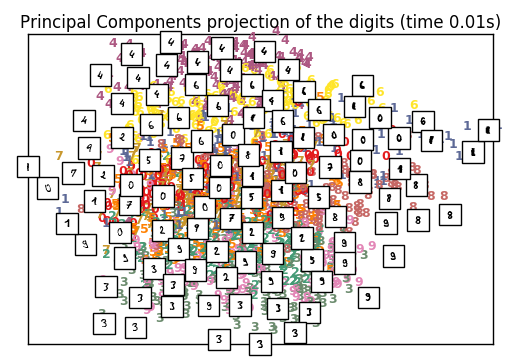
\includegraphics[scale=0.4]{tsne1.png}
	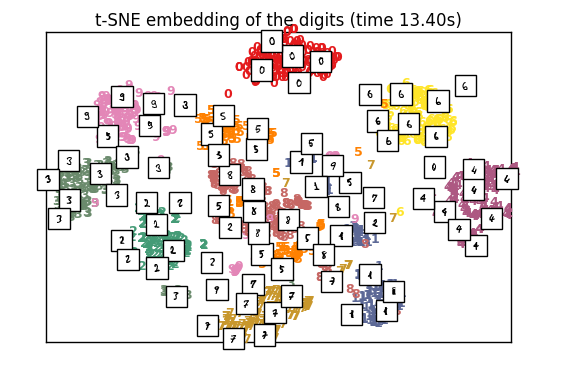
\includegraphics[scale=0.4]{tsne2.png}
\end{center}
Ici un exemple pour la classification de chiffres manuscrits. Les résultats sont bien meilleurs avec t-SNE mais hélas le temps de calcul est aussi bien plus long.
	
\end{document}